\documentclass[a4paper,french,bookmarks]{book}

\usepackage{booktabs}
\usepackage{minitoc}
\usepackage{./Structure/4PE18TEXTB}
\usepackage{proof}
\usepackage{pdfpages}

\usepackage{subfiles}

\makeatletter
\renewcommand*\l@section{\@dottedtocline{1}{1.8em}{3.5em}}
\renewcommand*\l@subsection{\@dottedtocline{2}{5.3em}{3.5em}}
\makeatother

\newboxans
\renewcommand{\thechapter}{\Roman{chapter}}
\renewcommand{\thesubsection}{\thesection.\Alph{subsection}}
\renewcommand{\thesubsubsection}{\thesubsection.\alph{subsubsection}}
\mtcsettitle{minitoc}{}
\setcounter{secnumdepth}{4}
\setcounter{tocdepth}{3}
\setcounter{minitocdepth}{3}

\newcommand{\Atom}{\mathop{\bcA_\text{tom}}\nolimits}
\DeclareMathOperator{\Reg}{Reg}
\DeclareDocumentCommand\FO{g}{\funlv{FO}{#1}}
\DeclareDocumentCommand\FV{g}{\funlv{FV}{#1}}
\DeclareDocumentCommand\BV{g}{\funlv{BV}{#1}}
\DeclareDocumentCommand\FP{g}{\funlv{FP}{#1}}
\DeclareDocumentCommand\th{g}{\funlv{th}{#1}}
\DeclareDocumentCommand\First{g}{\funlv{First}{#1}}
\DeclareDocumentCommand\Last{g}{\funlv{Last}{#1}}
\DeclareDocumentCommand\Fact{g}{\funlv{Fact}{#1}}
\DeclareDocumentCommand\NFact{g}{\funlv{NFact}{#1}}
\DeclareDocumentCommand\Loc{g}{\funlv{Loc}{#1}}

\newcommand{\chaptertoc}[0]{
    \begin{tcolorbox}[
        enhanced,
        frame hidden,
        sharp corners,
        detach title,
        spread outwards     = 5pt,
        halign              = center,
        valign              = center,
        borderline west     = {3pt}{0pt}{main20!50!main2!95!gray!90},
        coltitle            = main20!50!main2!95!gray!90, 
        interior style      = {
            left color      = main1white2!65!gray!11,
            middle color    = main1white2!50!gray!10,
            right color     = main1white2!35!gray!9
        },
        arc                 = 0 cm,
        title               = SOMMAIRE,
        boxrule             = 0pt,
        fonttitle           = \bfseries\sffamily,
        overlay             = {
            \node[rotate=90, minimum width=1cm, anchor=south,yshift=-0.8cm]
            at (frame.west) {\tcbtitle};
        }
    ]
        \begin{minipage}{0.83\linewidth}
            \sffamily
            \minitoc
        \end{minipage}
    \end{tcolorbox}
}

\begin{document}
    
    %==============================
    % METADONNEES
    %==============================
    
    \title{Cours d'Informatique de MPI* (2022-2023)}
    \author{SIAHAAN--GENSOLLEN Rémy}
    \date{\today}
    \hypersetup{
        pdftitle={Cours d'Informatique de MPI* (2022-2023)},
        pdfauthor={SIAHAAN--GENSOLLEN Rémy},
        pdflang={fr-FR},
        pdfsubject={MPI*, Cours d'Informatique},
        pdfkeywords={MPI*, Cours d'Informatique, 2022-2023}
        pdfstartview=
    }
    
    %==============================
    % MISE EN PAGE
    %==============================
    
    \titleformat{\chapter}[display]{\normalfont\huge\bfseries}{}{0pt}{
        \begin{tcolorbox}[
            enhanced,
            frame hidden,
            sharp corners,
            spread sidewards    = 5pt,
            halign              = center,
            valign              = center,
            interior style      = {color=main1!20},
            arc                 = 0 cm,
            fontupper           = \color{black}\sffamily\bfseries\huge,
            fonttitle           = \normalfont\color{white}\sffamily\small,
            top                 = 1cm, 
            bottom              = 0.7cm,
            title               = Chapitre \thechapter,
            attach boxed title to bottom center = {
                yshift=\tcboxedtitleheight/2,
            },
            boxed title style = {
                frame code={
                \path[left color=main2!95!gray!90,
                right color=main1!95!gray!90] 
                    ([xshift=-10mm]frame.north west) -- 
                    ([xshift=10mm]frame.north east) -- 
                    ([xshift=10mm]frame.south east) -- 
                    ([xshift=-10mm]frame.south west) -- 
                    cycle;
                },
                interior engine=empty
            }
        ]
            #1
        \end{tcolorbox}%
    }
    \titlespacing*{\chapter}{0pt}{-120pt}{-15pt}
    \titleformat{name=\chapter,numberless}[display]{\normalfont\huge\bfseries}
    {}{0pt}{
        \begin{tcolorbox}[
            enhanced,
            frame hidden,
            sharp corners,
            spread sidewards    = 5pt,
            halign              = center,
            valign              = center,
            interior style      = {color=main1!20},
            arc                 = 0 cm,
            outer arc           = 0pt,
            leftrule            = 0pt,
            rightrule           = 0pt,
            fontupper           = \color{black}\sffamily\bfseries\huge,
            enlarge left by     = -1in-\hoffset-\oddsidemargin, 
            enlarge right by    = -\paperwidth+1in+\hoffset +
            \oddsidemargin+\textwidth,
            width               = \paperwidth, 
            left                = 1in+\hoffset+\oddsidemargin, 
            right               = \paperwidth-1in-\hoffset -
            \oddsidemargin-\textwidth,
            top                 = 1cm, 
            bottom              = 1cm
        ]
            #1
        \end{tcolorbox}%
    }
    \titlespacing*{name=\chapter,numberless}{0pt}{-115pt}{0pt}
    
    %==============================
    % PREMIERE DE COUVERTURE
    %==============================

    \includepdf[pages={1},scale=1.15,offset=0mm -18mm]{CICover.pdf}
    
    %==============================
    % PAGE VIDE
    %==============================
    
    \pagestyle{empty}
    
    %==============================
    % PAGE DE COUVERTURE INTERNE
    %==============================
    
    \begin{titlepage}
	    \begin{center}
	        {\scshape SIAHAAN-{}-GENSOLLEN Rémy\par}
	        {\footnotesize avec l'aide de \textsc{DRISSI Rayan} et \textsc{SALOUM Gwendal}\par}
	        \vspace{2.5cm}
	        {\huge\sffamily Cours d'\par}
	        \vspace{0.1cm}
	        {\Huge\bfseries\sffamily INFORMATIQUE\par}
	        \vspace{1cm}
	        {\Large\emph{donné pendant mon année de \guill{spé'} en \emph{$\textsf{MPI}^\star$} à
	        Janson-de-Sailly}\\[2pt]\texttt{2022-2023}\par}
	        \vfill
	        {\large\EBGaramond Compilé le \today\par}
        \end{center}
    \end{titlepage}
    
    %==============================
    % PAGE VIDE
    %==============================
    
    \pagestyle{empty}\text{}\newpage
    
    %==============================
    % STYLE DES EN-TÊTES ET PIEDS DE PAGES
    %==============================
    
    \renewcommand\chaptermark[1]{\markboth{#1}{}}
    
    \fancypagestyle{intro}{
        \fancyhf{}
        \renewcommand{\headrulewidth}{0pt}
        \renewcommand{\footrulewidth}{0pt}\fancyfoot[RO,LE]{\GillSansMTMedium\color{white5}\thepage\;/\;\pageref{LastPage}}
        \fancyhead[LE]{\GillSansMTMedium\color{white5}\bfseries COURS D'INFORMATIQUE}
        \fancyhead[RE]{\GillSansMTMedium\color{white5}Avant-propos}
        \fancyhead[LO]{\GillSansMTMedium\color{white5}\rightmark}
        \fancyhead[RO]{\GillSansMTMedium\color{white5}$\textbf{MPI}^\star$ 2022-2023 \quad Janson-de-Sailly}
    }
    
    \fancypagestyle{toc}{
        \fancyhf{}
        \renewcommand{\headrulewidth}{0pt}
        \renewcommand{\footrulewidth}{0pt}\fancyfoot[RO,LE]{\GillSansMTMedium\color{white5}\thepage\;/\;\pageref{LastPage}}
        \fancyhead[LE]{\GillSansMTMedium\color{white5}\bfseries COURS D'INFORMATIQUE}
        \fancyhead[RE]{\GillSansMTMedium\color{white5}Table des matières}
        \fancyhead[LO]{\GillSansMTMedium\color{white5}\rightmark}
        \fancyhead[RO]{\GillSansMTMedium\color{white5}$\textbf{MPI}^\star$ 2022-2023 \quad Janson-de-Sailly}
    }
    
    \fancypagestyle{plain}{
        \fancyhf{}
        \renewcommand{\headrulewidth}{0pt}
        \renewcommand{\footrulewidth}{0pt}\fancyfoot[RO,LE]{\GillSansMTMedium\color{white5}\thepage\;/\;\pageref{LastPage}}
        \fancyhead[LE]{\GillSansMTMedium\color{white5}\bfseries COURS D'INFORMATIQUE}
        \fancyhead[RE]{\GillSansMTMedium\color{white5}Chapitre \thechapter : \nouppercase{\leftmark}}
        \fancyhead[LO]{\GillSansMTMedium\color{white5}\nouppercase{\rightmark}}
        \fancyhead[RO]{\GillSansMTMedium\color{white5}$\textbf{MPI}^\star$ 2022-2023 \quad Janson-de-Sailly}
    }
    
    %==============================
    % PREFACE 
    %==============================
    
    \chapter*{Avant-propos}
    \thispagestyle{intro}
    \addcontentsline{toc}{chapter}{Avant-propos}
    
    \text{\Large\EBGaramond\itshape À tout lecteur potentiel, quelques mots...}\newline\newline\newline
    
    \begin{center}
        \begin{minipage}{0.85\linewidth}
            \large \qquad Comme son nom peut l'indiquer, cet ouvrage est la compilation de notes de cours d'informatique dispensés par M. Antony \textsc{Lick} durant mon année de \guill{spé'} en \textsf{MPI*} à \textit{Janson-de-Sailly} (année académique 2022-2023). De ce fait, certaines parties risquent d'être elliptiques, lacunaires, voire inexistantes, alors qu'elles seraient vitale à la compréhension du cours. Elles pourraient de plus être erronées, ou rédigées maladroitement, et induire en erreur.  Ainsi, j'aviserai tout lecteur potentiel à faire preuve de prudence lors du parcours de ce texte, et à ne pas hésiter à en vérifier le contenu par lui-même au moindre doute.\newline
            
            J'essaierai le plus possible de détailler et d'enrichir le contenu de ce livre au cours de l'année, que ce soit à l'aide de mes cours de première année, d'autres ouvrages, ou de recherches en général.
            
            %J'essaierai par ailleurs de détailler et d'enrichir le plus possible son contenu au fil de l'année, à l'aide de mes cours de première année, d'autres ouvrages et de recherches en général. La rédaction de ce cours constitue un important projet, d'autant plus que j'en mène un similaire pour les enseignements de mathématiques et de physique cette année. C'est un travail qui peut s'avérer extrêmement chronophage, aussi risque-t-il d'être rarement mené jusqu'au bout.\newline
    
            %\qquad Je ne prétends à aucun moment être enseignant, et ce livre reste avant tout destiné à mon usage personnel, aussi j'aviserai tout lecteur potentiel à faire preuve de prudence lors du parcours de ce texte, à ne pas hésiter à en vérifier le contenu par lui même. Il est très probable que de multiples erreurs (en tout genre) se soient glissés durant la rédaction, que je n'aurait su repérer, ou que le manque de temps empêche la correction. N'hésitez d'ailleurs pas à me le signaler, ou à me faire part de vos remarques en général.\newline
    
            %\qquad J'espère enfin, et malgré les points exprimés précédemment, que ce cours pourra avoir une quelconque utilité à ceux qui s'y aventureraient, que sa lecture et son style en seront agréable (la mise en page et la composition graphique en général sont de ma conception personnelle, enrichie par les retours de mes camarades, et le fruit de plusieurs mois d'apprentissage de \LaTeX) et enrichissante.\newline\newline\newline\text{}
        \end{minipage}
    \end{center}
    
    \hfill{\large\textsc{SIAHAAN-{}-GENSOLLEN Rémy}}
    
    \pagestyle{intro}
    
    %==============================
    % TABLE DES MATIERES
    %==============================

    %\newpage
    \dominitoc\nomtcrule 
    {\sffamily\tableofcontents}\mtcaddchapter\pagestyle{toc}
    
    %\cleardoublepage
    
    %==============================
    % COURS
    %==============================
    
    \pagestyle{plain}
    
    \chapter{Logique et systèmes de preuve}
    
    \subfile{chapitre1}
    
    \begin{definition}{Min-terme}{}
        Soient \hg{$I$ un ensemble fini ou dénombrable d'indices} et \hg{$\bcV = \ens{v_i}_{i \in I}$ un ensemble de variables propositionnelles}. On appelle \hg{min-terme sur $\bcV$} la \hg{conjonction $\displaystyle\bigwedge_{i \in I} a_i$ des littéraux de $\ens{a_i \enstq a_i \in \ens{v_i, \neg v_i}}_{i \in I}$}.
    \end{definition}
    %
    On donne ci-dessous quelques exemples de mini-termes.
    %
    \begin{example}{}{}
        On considère $I = \iint{1, 3}$ et $\bcV = \ens{v_1, v_2, v_3}$ :
        \begin{enumerate}
            \itt $\hg{\neg v_1 \land v_2 \land \neg v_3}$ est un min-terme.
            
            \itt $\hg{v_1 \land \neg v_2}$ et $\hg{\neg v_1 \land v_2 \land v_1}$ ne sont \bf{pas} des min-termes.
        \end{enumerate}
    \end{example}
    %
    L'utilité des min-termes réside dans la propriété suivante :
    %
    \begin{property}{Table de vérité d'un min-terme}{}
        Soit \hg{$\bcV$ un ensemble fini ou dénombrable de variables propositionnelles}. \hg{A chaque min-terme $m$} sur $\bcV$ \hg{correspond une unique valuation $\bcv_m$} sur $\bcV$ telle que \hg{$\bcv_m \vDash m$}, et \hg{réciproquement}.
    \end{property}
    %
    \begin{nproof}
        Soient $I$ un ensemble fini ou dénombrable d'indices, $\bcV = \ens{v_i}_{i \in I}$ un ensemble de variables propositionnelles et $m$ un min-terme sur $\bcV$. Soient $\bcv$ une valuation sur $\bcV$ telle que $v\p{m} = 1$ et $\ens{a_i \enstq a_i \in \ens{v_i, \neg v_i}}_{i \in I}$ tels que $m = \displaystyle\bigwedge_{i=1}^n a_i$.
        %
        \[ 1 = \bcv\p{m} = v\p{\bigwedge_{i \in I} a_i} = \prod_{i \in I} \bcv\p{a_i} = \prod_{\substack{i \in I\\a_i = v_i}} v\p{v_i} \prod_{\substack{i \in I\\a_i = \neg v_i}} \p{1 - \bcv\p{v_i}} \qquad\text{donc}\quad \forall i \in I\quad \bcv\p{a_i} = \left\lbrace\begin{array}{ll}
            1 &\text{si} \ a_i = v_i  \\
            0 &\text{si} \ a_i = \neg v_i 
        \end{array}\right.\]
        %
        Ainsi $\bcv$ est entièrement déterminée, d'où l'unicité. Pour l'existence, $\bcv$ ainsi décrit convient. Il n'existe donc qu'une unique valuation satisfaisant $m$. Réciproquement, on pose $\ens{a_i \enstq \begin{array}{ll}
            a_i = v_i &\text{si} \ \bcv\p{a_i} = 1  \\
            a_i = \neg v_i &\text{si} \ \bcv\p{a_i} = 0 
        \end{array}}_{i \in I}$. On a facilement que le min-terme $m_\bcv = \displaystyle\bigwedge_{i \in I} a_i$ est alors le seul satisfait par $\bcv$. 
    \end{nproof}
    %
    Les min-termes permettent d'obtenir une forme normale disjonctive \guill{canonique}, au sens de l'unicité :
    %
    \begin{corollary}{Existence et unicité de la FNDC}{}
        Soit \hg{$\bcV$ un ensemble fini ou dénombrable de variables propositionnelles}, \hg{$\Gamma$ un ensemble de formules propositionnelles} à variables dans $\bcV$ et \hg{$\varphi \in \Gamma$ une formule} logique de $\Gamma$.
        %
        \[ \text{\hg{Il existe une unique disjonction de min-termes différents logiquement équivalente à $\varphi$}.} \]
    \end{corollary}
    %
    \begin{nproof}
        Soit $\bcV$ un ensemble fini de variables propositionnelles, $\Gamma$ un ensemble de formules propositionnelles à variables dans $\bcV$ et $\varphi \in \Gamma$ une formule logique de $\Gamma$. Pour toute valuation $\bcv$ sur $\bcV$, on note $m_\bcv$ l'unique min-terme sur $\bcV$ satisfait par $\bcv$. On pose alors $\psi = \displaystyle\bigvee_{\bcv \in \ens{\bcv \enstq \bcv \vDash \phi}} m_\bcv$. Par définition de l'équivalence logique, on a directement $\varphi \equiv \psi$.\medskip
        
        Pour l'unicité, supposons $\psi'$ une disjonction de min-termes équivalente logiquement à $\varphi$. Soit $m$ un min-terme sur $\bcV$ et soit $\bcv$ l'unique valuation sur $\bcV$ satisfaisant $m$, d'où $m = m\bcV$. 
        
        Si $\bcv \vDash \varphi$, alors $m = m_\bcv$ est dans $\psi$. Si $\bcv \not\vDash \varphi$, alors $m = m_\bcv$ n'est pas dans $\psi$. Par contraposée, $m$ est dans $\psi$ si et seulement s'il est dans $\psi'$. On a bien unicité.
    \end{nproof}
    
    On remarque alors que cette disjonction de min-termes est une forme normale disjonctive, d'où :
    %
    \begin{definition}{Forme normale disjonctive canonique}{}
        Soit \hg{$\bcV$ un ensemble fini ou dénombrable de variables propositionnelles}, \hg{$\Gamma$ un ensemble de formules propositionnelles} à variables dans $\bcV$ et \hg{$\varphi \in \Gamma$ une formule} logique de $\Gamma$. On appelle \hg{forme normale disjonctive canonique de $\varphi$} l'\hg{unique disjonction de min-termes différents logiquement équivalente à $\varphi$}.
    \end{definition}
    
    \chapter{Langages formels et théorie des automates}
    
    Généralement, la résolution d'un problème passe par la compréhension de celui-ci, puis par différentes méthodes mathématiques, ce que l'on pourrait généralement appeler \textit{calcul} (que ce soit du calcul avec des nombres, avec des lettres, ou des objets plus abstraits). Savoir si un tel calcul peut être fait et dans quelles conditions ouvre d'ailleurs la question de la \textit{calculabilité}. La branche de l'informatique théorique qui étudie cette formalisation des mécanismes mathématiques s'appelle la \textit{théorie des automates}. Assez récente, elle n'émerge comme une discipline indépendante que dans la deuxième moitié du \textsc{XX}\ieme~siècle, sous l'impulsion des travaux de scientifiques comme Claude \textsc{Shannon}, John \textsc{von Neumann}, Edward \textsc{Moore}, Stephen \textsc{Kleene}, \dots 
    
    Le principe de la théorie des automates est de convertir un \guill{problème} en un langage formel, dans lequel l'analyse de certains éléments peut conduire à la résolution de ce problème. Ses applications sont nombreuses, que ce soit en intelligence artificielle, pour le traitement de texte, en biologie, ou toujours en informatique (les automates sont à la base de la théorie de la complexité). Un \textit{automate} 
    
    Dans ce chapitre, on s'intéressera aux langages formels 

    Le but de ce chapitre est d'étudier formellement divers ensembles de
    chaînes de caractères, ayant des propriétés intéressantes du point de vue informatique.
    
    \chaptertoc
    
    \section{Langages réguliers}
    
    \subsection{Alphabets, mots et langages}
    
    La première composante essentielle à un langage est son alphabet. On a une compréhension assez intuitive de ce concept, ne serait-ce qu'en pensant à l'alphabet latin, l'alphabet grec, l'alphabet cyrillique, \etc. On voit donc un \guill{alphabet} comme un \textit{ensemble} de différents \textit{symboles}, qu'on appelle aussi souvent \textit{lettres}. En informatique, on reprend cette notion, en la définissant ainsi :
        
    \begin{definition}{Alphabet, lettres}{}
        On appelle \hg{alphabet} un \hg{ensemble non vide et fini}. On appelle \hg{lettres} ou \hg{symboles} les éléments de cet ensemble.
    \end{definition}
    %
    \begin{notation}
        On désignera usuellement par \hg{$\Sigma$ un alphabet}, et par \hg{$a, b, c, \dots$ les lettres} de $\Sigma$.
    \end{notation}
    
    On donne ci-dessous quelques exemples d'alphabets utilisés en informatique :
    
    \begin{example}{}{}
        \begin{enumerate}
            \itt On a \hg{$\Sigma = \ens{0, 1}$} l'\textit{alphabet} des \hg{nombres en binaire}.
            
            \itt On a $\hg{\Sigma = \ens{a, b, c, \dots, z}}$ l'\textit{alphabet} \hg{latin} (ici constitué des \textit{lettres} minuscules non accentuées).
            
            \itt On a l'\textit{alphabet} des \hg{caractères \texttt{Unicode}}.
        \end{enumerate}
    \end{example}
    
    Une fois les notions d'alphabet et de lettre introduites, on peut considérer la notion de mot, qu'on peut voir comme une suite finie de lettres d'un alphabet :
    
    \begin{definition}{Mot, longueur}{}
        Soient \hg{$\Sigma$} un \hg{alphabet} et \hg{$n \in \bdN$} un \hg{entier naturel}.
        %
        \begin{enumerate}
            \itast On appelle \hg{mot} (sur $\Sigma$) un \hg{$n$-uplet $u \in \Sigma^n$}.
            
            \itast On appelle \hg{longueur} du mot \hg{$u \in \Sigma^n$} l'\hg{entier $n$}.
            
            \itast On appelle \hg{mot vide} l'unique mot \hg{$\emptyset \in \Sigma^0$} de \hg{longueur nulle}.
        \end{enumerate}
    \end{definition}
    
    \begin{notation}
        \begin{enumerate}
            \itt On désigne généralement un \hg{mot} par \hg{$u$}, \hg{$v$}, \hg{$w$}, \hg{$x$}, \hg{$y$} ou \hg{$z$}.
            
            \itt On peut représenter le mot \hg{$u = \p{a_1, a_2, \dots, a_n} \in \Sigma^n$} à l'aide ses lettres, selon \hg{$u = a_1a_2\cdots a_n \in \Sigma^\star$}. 
            
            \itt Lorsqu'un \hg{mot} n'est formé \hg{que d'une lettre}, on \hg{identifiera les deux}.
            
            \itt L'\hg{ensemble des mots} sur $\Sigma$ est également noté \hg{$\Sigma^\star$}.
            
            \itt La \hg{longueur du mot $u \in \Sigma^\star$} est notée \hg{$\mod{u}$}.
            
            \itt Le \hg{mot vide} est généralement désigné par \hg{$\epsilon$}.
        \end{enumerate}
    \end{notation}
    
    On donne donc ci-dessous quelques exemples d'ensembles de mots :
    %
    \begin{example}{}{}
        \begin{enumerate}
            \itt Considérons l'\hg{alphabet $\Sigma = \ens{a, b, c}$}, on a l'\hg{ensemble des mots} de longueur inférieure ou égale à $2$ suivant :
            %
            \[ \hg{\ens{u \in \Sigma^\star \vphantom{\dfrac{-}{-}}\enstq \mod{u} \leq 2} = \ens{\epsilon, a, b, c, aa, ab, ac, ba, bb, bc, ca, cb, cc}} \]
            
            \itt Considérons un microprocesseur de \texttt{64 bits}. On a l'\hg{alphabet $\Sigma = \ens{0, 1}$}.
            
            L'ensemble des \hg{valeurs possibles pour un registre de calcul} est \hg{$\ens{\vphantom{\dfrac{}{}}u \in \Sigma^\star \enstq \mod{u} = 64}$}. 
        \end{enumerate}
    \end{example}
    
    On peut dès lors commencer à donner une structure aux notions précédemment définies. Une première opération usuelle est le fait de \guill{regrouper} deux mots, \ie la concaténation :
    
    \begin{definition}{Concaténation}{}
        Soient \hg{$\Sigma$} un \hg{alphabet}, \hg{$\p{n, m} \in \bdN^2$} deux \hg{entiers}, \hg{$u = a_1\dots a_n \in \Sigma^\star$} un \hg{mot de longueur $n$} et \hg{$v = b_1\dots b_n \in \Sigma^\star$} un \hg{mot de longueur $m$}. On appelle \hg{concaténation de $u$ et $v$} le \hg{mot $w = a_1\dots a_nb_1 \dots b_n$ de longueur $n + m$}. 
    \end{definition}{}{}
    
    \begin{notation}
        La \hg{concaténation de $u$ et $v$} est généralement notée \hg{$u \cdot v$} ou \hg{$uv$}.
    \end{notation}
    
    Immédiatement, il vient :
    %
    \begin{property}{Associativité et neutre de la concaténation}{}
        Soit \hg{$\Sigma$} un \hg{alphabet}. La \hg{concaténation $\cdot$} est une \hg{loi de composition interne}, \hg{associative} et \hg{de neutre $\epsilon$ sur $\Sigma^\star$}.
    \end{property}
    %
    \begin{nproof}
        Soit $\Sigma$ un alphabet, $\p{n, m, p} \in \bdN^3$ trois entiers, et $u = a_1\cdots a_n \in \Sigma^\star$, $v = b_1\cdots b_m \in \Sigma^\star$, $w = c_1\cdots c_p \in \Sigma^\star$ trois mots sur $\Sigma$.
        %
        \begin{enumerate}
            \itt $uv \in \Sigma^\star$ est un mot, donc la concaténation $\cdot$ est une loi de composition interne de $\Sigma^\star$.
            
            \itt $u\epsilon = a_1\cdots a_n = \epsilon u = u$, donc $\epsilon$ est un élément neutre de la concaténation $\cdot$.
            
            \itt On a :
            %
            \[ \p{uv}w = \p{a_1\cdots a_nb_1\cdots b_m}c_1 \cdots b_p = a_1\cdots a_nb_1\cdots b_mc_1\cdots b_p = a_1 \cdots a_n\p{b_1 \cdots b_mc_1 \cdots b_p} = u\p{vw}\]
        \end{enumerate}
        %
        \qquad\quad Donc la concaténation $\cdot$ est associative.
    \end{nproof}
    
    Ainsi, $\Sigma^\star$ muni de la concaténation $\cdot$ correspond une structure algébrique particulière : on parle du \textit{monoïde} $\p{\Sigma^\star, \cdot}$.
    %
    On peut maintenant considérer l'opération qui consiste en la concaténation répétée d'un mot avec lui-même :
    
    \begin{definition}{Puissance}{}
        Soient \hg{$\Sigma$} un \hg{alphabet}, \hg{$n \in \bdN$} un \hg{entier} et \hg{$u \in \Sigma^\star$} un \hg{mot} sur $\Sigma$. On appelle \hg{puissance $n$-ième de $u$} le \hg{$n$-ième itéré} de \hg{$u$} par la \hg{concaténation}.\medskip
        
        On pourra parler de \hg{puissance carré} pour la \hg{puissance $2$-ième}, de \hg{puissance cubique} pour la \hg{puissance $3$-ième}, \etc.
    \end{definition}
    %
    \begin{notation}
        Le \hg{$n$-ième itéré de $u$} sera généralement noté \hg{$u^n = \underbrace{u \cdot u \cdot \dots \cdot u}_{n \ \text{fois}}$}.
    \end{notation}
    
    Avec cette notation, on peut redonner la définition sous la forme suivante :
    %
    \begin{enumerate}
        \begin{minipage}{0.5\linewidth}
            \itt $u^0 = \epsilon$
        \end{minipage}
        %
        \begin{minipage}{0.5\linewidth}
            \itt pour tout entier $k \in \bdN$, $u^{k+1} = u \cdot u^k$.
        \end{minipage}
    \end{enumerate}
    
    On donne ci-dessous un exemple d'utilisation de la concaténation et des puissances :
    
    \begin{example}{}{}
        On considère l'\hg{alphabet $\Sigma = \ens{a, b, c}$}, le \hg{mot $u = ab \in \Sigma^\star$} et le \hg{mot $v = cab \in \Sigma^\star$}. On a :
        %
        \begin{enumerate}
            \itt \hg{$uv = u \cdot v = abcab \in \Sigma^\star$} (concaténation de $u$ et $v$).
            
            \itt \hg{$v^2 = v \cdot v = cabcab \in \Sigma^\star$} (puissance carré de $v$).
            
            \itt \hg{$vu^2 = v \cdot u^2 = v \cdot u \cdot u = cababab \in \Sigma^\star$} (concaténation de $v$ et de la puissance carré de $u$).
            
            \itt \hg{$c\p{ab}^3 = c \cdot \p{ab}^3 = cababab \in \Sigma^\star$} (concaténation du mot-lettre $c$ et de la puissance cubique du mot $ab$).
            
            \itt \hg{$a^4b^2c^2 = aaaaabbcc \in \Sigma^\star$} (concaténation de puissances des mot-lettre $a$, $b$ et $c$).
        \end{enumerate}
    \end{example}
    
    Inversement, on peut voir tout mot comme la concaténation de plusieurs \guill{sous-mots}. Même dans le cas d'un simple mot d'une lettre, on peut le voir comme la concaténation de lui-même avec le mot vide $\epsilon$. Ainsi on définit : 
    
    \begin{definition}{Préfixe, suffixe}{}
        Soient \hg{$\Sigma$} un \hg{alphabet} et\hg{$\p{u, v, w} \in \p{\Sigma^\star}^3$} trois \hg{mots} sur $\Sigma$ tels que \hg{$w = u \cdot v = uv$}. On dit que :
        %
        \begin{enumerate}
            \begin{minipage}{0.5\linewidth}
                \itast \hg{$u$ est un préfixe de $w$}
            \end{minipage}
            %
            \begin{minipage}{0.5\linewidth}
                \itast \hg{$v$ est un suffixe de $w$}
            \end{minipage}
        \end{enumerate}
    \end{definition}
    
    On notera que tout mot non vide possède au moins deux préfixes et deux suffixes distincts : $\epsilon$ et lui-même. Pour un mot $u \in \Sigma^\star$ on peut en effet toujours écrire $u = \epsilon\cdot u = u \cdot \epsilon$.
    
    \begin{example}{}{}
        On considère l'\hg{alphabet $\Sigma = \ens{a, b}$}. Les \hg{préfixes du mot $abbab \in \Sigma^\star$} sont :
        %
        \[ \hg{\epsilon,\ a,\ ab,\ abb,\ abba,\ abbab} \]
    \end{example}
    
    On peut 
    
    \begin{definition}{acteur}{}
        Soit $w \in \Sigma^\star$.
        On dit que u est un facteur de w si :
        $\exists (v,v') \in (\Sigma^\star)^2$ tel que $w = v u v'$
        
    \end{definition}
    
    \begin{definition}{Sous-mot}{}
        Soit $w=a_1 \dots a_n$ un mot sur $\sigma$.
        Un \hg{sous-mot} est un mot de la forme $a_{i_1} \dots a_{i_k}$ avec $1 \leq i_1 < \dots < i_k \leq n$
        
    \end{definition}
    
    \begin{warning}{}{}
        Ne pas confondre "facteur" et "sous-mot".
        \begin{enumerate}
            \itt bca est un facteur de w.
        \end{enumerate}
    \end{warning}
    
    \begin{example}{}{}
        $w=abcabc$
        \begin{enumerate}
            \itt $bca$ a est un sous mot de $w$
            \itt $abab$ est un sous mot de $w$
            \itt $cac$ est un sous mot de $w$
            
            
        \end{enumerate}
        
        On remarque que les relations "être préfixe, suffixe, facteur, sous-mot" sont des \hg{relations bien fondées} sur $\sigma^\star$.
        
    \end{example}
    \begin{definition}{mot miroir}{}
        \begin{enumerate}
            \itt on appelle mot miroir de w et note $w^R$
        le mot $w^r =  a_1 \dots a_n$
            \itt un palindrome est un mot qu'on peut lire dans les deux sens tel que $w=w^R$
            
            
            
        \end{enumerate}
        
    \end{definition}
    
    \begin{definition}{Langage}{}
        Un langage $L$ sur un alphabet $\Sigma$ et un sous ensemble $\Sigma^*$ 
    \end{definition}
    
    \begin{example}{}{}
        On prend $\Sigma = \ens{a, b, c}$.
        %
        \begin{enumerate}
            \itt $L_1 = \ens{abc, bca, acb}$ est un langage fini.
            
            \itt $L_2 = \ens{ab^nc \enstq n \in \bdN}$ est le langage infini des mots commençant par $a$; suivi d'une suite (de taille arbitraire) de $b$, et finissant par $c$.
            
            \itt $L_3 = \ens{a^n \enstq n \in \bdP}$
        \end{enumerate}
    \end{example}
    
    \begin{notation}
        On note $\overline{L}$ le complémentaire de L :
        $\overline{L} = \Sigma^* \backslash L$
    \end{notation}
    
    \begin{definition}{Concaténation de deux langages}{}
        Soit $L_1 et L_2$ des langages sur $\Sigma$.
        Le langage \hg{concaténation}  de $L_1$ et $L_2$, noté $L_1 L_2$, est défini par :
        $L_1 L_2 = \ens{\omega \enstq \exists u \in L_1, \exists v \in L_2, \omega = uv}$
    \end{definition}
    
    \begin{example}{}{}
        $L_1 = \ens{aa, ab, bc} ; L_2 = \ens{\epsilon, a, abc}$
        $L_1 L_2 = \ens{aa, ab, bc, aaa, aba, bca, aaabc, ababc, bcabc}$
    \end{example}
    
    \begin{definition}{Puissance d'un language }
        Soit $L \subset \Sigma^*$, Soit $n\in \bcN$  
        
        
        Le langages $L^n$ est definit par récurrence sur $n$
        \begin{enumerate}{}{}
            
            \itt $L^0 = \ens{ \varepsilon}$
            
            \itt %lol itt comme un jour d'itt 
                $L^n+1 = L * L^n $ pour $n \geq 0$ 
                
        \end{enumerate}{}
        
    \end{definition}
    
    \begin{warning}{}{}
        \begin{enumerate}
            \itast Ne pas confondre $\emptyset$ et $\ens{\epsilon}$
            
            \itast Ne pas confondre $L^n$ et $\ens{u^n \enstq u \in L}$
        \end{enumerate}
    \end{warning}
    
    \begin{definition}{Étoile de Keeme}{}
        Soit \hg{$L \subset \Sigma^\star$}. On appelle \hg{étoile de \textsc{Kleene} de $L$} le langage \hg{$\displaystyle \bigcup U_{n \in \bdN} L^n$}.
    \end{definition}
    
    \begin{notation}
        L'\hg{étoile de \textsc{Kleene} de $L$} est généralement notée \hg{$L^\star$}.
    \end{notation}
    
    On remarque que
    \begin{enumerate}
        \itt c'est de la que vient la notation $\Sigma^\star$
        \itt On note parfois $L^+ = \bigcup_{n > 0} L^n$
    \end{enumerate}
    
    \begin{definition}{langage miroir}{}
        Soit $L \subset \Sigma^\star$. On appelle langage mirroir de L le langage $L^r$ défini par $L^r = \ens{\omega^r \enstq \omega \in L}$
        
    \end{definition}
    
    \subsection{Langage réguliers, expression régulières}
    
    \begin{definition}{Langage réguliers}{} 
        Soit $\Sigma$ un alphabet. L'ensemble des langages réguliers sur $\Sigma$ (ou langages rationnels sur $\Sigma$) est défini inductivement par: 
        \begin{enumerate}
            \itast $\emptyset$ est un langage régulier
            
            \itast  Pour tout $a \in \Sigma$, $\ens{a}$ est régulirer ;
            
            \itast si $A$ et $B$ sont des langages réguliers, alors $A \cup B$, $AB$ et $A^\star$ sont réguliers.
            
        \end{enumerate}
    \end{definition}
    %
    \begin{notation}
        On note $\Reg_\Sigma$ l'ensemble des langages réguliers sur $\Sigma$.
    \end{notation}
    
    Parfois, on inclut dans la définition précédente que $\ens{\epsilon}$ est régulier. Ceci est en fait redondant car $\ens{\epsilon} = \emptyset^\star$
    
    \begin{definition}{Expression régulière}{}
        
        Une expression régulière sur un alphabet $\Sigma$ ou expression rationnelle est définie inductivement 
        %
        \begin{enumerate}
            \itast $\emptyset$ et $\epsilon$ sont*µ des expressions régulières.
            
            \itast pour tout $e \in \Sigma$, $e$ est une expression régulière.
            
            \itt si $r_1 et r_2$ sont deux expression réguliere 
                \begin{enumerate}
                    \itt $r_1 | r_2$ est une expression réguliere 
                    
                    \itt $r_1, r_2$ est une expression régulière
                    
                    \itt $r_1^* $ est une expression régulière
                \end{enumerate}
        \end{enumerate}
    \end{definition}
    
    On notera que les règles de priorité sont ${}^\star > \cdot > \vert$.
    
    
    \begin{definition}{Langage d'une expression reguliere}{}
        Soit r une expression reguliere sur $\Sigma$
        
        le langage de l'equation r, noté $\bsL(r)$, est defini par induction structurelle sur r≠
        
        
        \begin{enumerate}
            \itt $\bsL\p{\emptyset} = \ens{\emptyset}$
            \itt $\bsL\p{\epsilon} = \ens{\epsilon}$
            \itt $\forall a \in \Sigma, \bsL\p{a} = \ens{a}$
            \itt $\bsL\p{r_1 \enstq r_2} = \bsL \p{r_1} \cup \bsL \p{r_2}$
            \itt $\bsL\p{r_1 r~……∞,_2} = \bsL \p{r_1} \bsL \p{r_2}$
            \itt $\bsL\p{r^\star} = \bsL \p{r}^\star$ 
        \end{enumerate}
    \end{definition}{}
    
    \begin{example}{}{}
        \begin{enumerate}
            \itt $mpi^\star : \ens{mpi \dots i}$
            \itt $\p{mpi}^\star : \ens{mpimpi \dots mpi}$
            
            \itt L'ensemble des nombres en base 2 sans zéro non significatif est reconnu par
            $0 \vert 1 \p{0 \vert 1}^\star$
            
            \itt $0^\star 1 0^\star 1 0^\star 1 0^\star$ décrit le langage des mots sur $\Sigma = \ens{0, 1}$ contenant exactement trois 1.
        
            \itt $\p{a \vert b \vert c \vert \dots \vert z \vert .\vert-}^\star @ \p{a \vert \dots \vert z \vert -}.\p{com \vert fr \vert \dots}$
            est l'ensemble des adresses mails syntaxiquement correctes.
        \end{enumerate}
    \end{example}
    
    \begin{enumerate}
        \itt En anglais, le terme \textit{regular expression} est souvent abrégé en \textit{regex}.
        
        \itt sous \textit{Linux}, l'outil \texttt{grep} permet de rechercher un motif dans des fichiers a l'aide d'expression régulières :
        %
        \[ \text{\sffamily\textbf Globally \textbf regular \textbf expression \textbf print }\]
        
        L'outil \texttt{grep} utilise une syntaxe étendue (\textsf{POSIX}) pour décrire les expressions régulières (\cf TP1).
        
    \end{enumerate}
    
    \section{Automates finis}
    
    Les automates sont des objets calculatoires fondamentaux a l'informatique.
    Il en existe de nombreusses variantes, selon le domaine d'application 
    \begin{enumerate}
        
        \itt automates finis 
        \itt automates à pile 
        \itt automates d'arbre 
        \itt automates àcompteurs 
        \itt automates temporisés 
        
    \end{enumerate}
    
    Voici quelque applications
    
    \begin{enumerate}
        \itt analayse de texte 
        \itt blabla  blabla 
        \itt blablab blabla 
        \itt blablablbla
        
        \itt IA 
        
        \itt ...
        
    \end{enumerate}
    
    \subsection{Automates déterministes}
    
    \begin{definition}{automates fini déterministes complet}{}
        
        Un \hg{automates fini déterministe complet} (ou CDFA) 
        
        est un quintuplet $\bcA$ = $Q,\Sigma, q_0, F, \sigma$
        \begin{enumerate}
            \itt $Q$ est un ensemble fini d'\hg{états}
            \itt $\Sigma est un alphabet$
            \itt $q_0 \in Q$ est l'\hg{état initial}
            \itt $F \subset Q$ est l'ensemble des \hg{états finaux} (\hg{ou acceptants})
            \itt $\sigma :  Q  *  \Sigma -> Q $est une fonction totale, appeler fonction de l'automate.   
        
        \end{enumerate}
    
    \end{definition}
    
    \begin{example}{}{}
        $\bsA_{bin} = \p{\ens{q_0, q_1, q_2, q_\bot}, \ens{0, 1}, q_0, \ens{q_1, q_2}, \delta_{bin}}$
        
        avec $\sigma_{bin} :$
        \begin{enumerate}
            \itt $\p{q_0, 0} \to q_1$
            \itt $\p{q_0, 1} \to q_2$
            \itt $\p{q_1, 0} \to q_\bot$
            \itt $\p{q_1, 1} \to q_\bot$
            \itt $\p{q_2, 0} \to q_2$
            \itt $\p{q_2, 1} \to q_2$
            \itt $\p{q_\bot, 0} \to q_\bot$
            \itt $\p{q_\bot, 1} \to q_\bot$
        \end{enumerate}
    \end{example}
    \begin{notation}
        représentation d'un automates par un graphe
        
        \begin{enumerate}
            \itt chaque état est un sommet du graphe (q)
            
            \itt l'état initiale est indiqué par une flèche entrante: ($--> q_0$)
            
            \itt si $q_f \in F$, il est entouré 2 fois.
            
            \itt si $\delta \p{q_1, a} = q_2$ on a un arc.
            
            
        \end{enumerate}
        
        
    \end{notation}
     
    \begin{example}{}{}
        L'automate $\Atom$ peut être représenté comme suit :
        
        \begin{tikzpicture}
            \draw[->] (0, 0) -- (1, 0);
            
            \node[draw, circle] at (1, 0) {$q_0$} ;
        \end{tikzpicture}
        
    
        
    \end{example}
    \begin{definition}{chemin}{}
        Soit $\bcA = (Q,\Sigma, q_0, F, \delta)$ sur CDFA.
        
        
        Soit $v = a_1 \dots a_n  \in \Sigma^\star$ 
        
        Le chemin est dit \hg{acceptant} si $r_0 = q_0 et r_a \in F$
        On dit que $\bsA$ \hg{reconnaît} (ou \hg{accepte}) le mot $v$ s'il existe un chemin l'acceptant par v dans $\bsA$
        
    \end{definition}
    
    \begin{notation}
        \begin{enumerate}
            \itt On note $r_0\lima{a_1} r1 \lima{a_2} \dots r_{n - 1} \lima{a_n} r_n$ un chemin.
            \itt Si on ne souhaite pas spécifier tout les états intermédiaires on note $r_0 \lima{v} r_n$ lorsqu'il n'y a pas de doute sur $\bsA$.
        \end{enumerate}
    \end{notation}
    
    \begin{example}{}{}
        \begin{enumerate}
            \itt $v = 0 : q_0 \lima{0} q_1 \in F$ donc 0 est accepté par $\bsA_{bin}$.
            \itt $v = 101 : q_0 \lima{1} q_2 \lima{0} q_2 \lima{1} q_2 \in F$ Donc 101 est accepté
            \itt $v = 010 : q_0 \lima{0} q_1 \lima{1} q_\bot \lima{0} q_\bot \notin F$
        \end{enumerate}
    \end{example}
    
    On remarque que si $q \in Q$ est tel que :$\forall a \in \Sigma, \delta \p{q, a} = q$, on dit que $q$ est un état absorbant.
    
    \begin{example}{}{}
        $q_1 et q_2$ sont des états absorbants de $\bsA_{bin}$.
    \end{example}
    
    \begin{definition}{Langage d'un automate}{}
        Soit $\bsA$ un automate. Le langage de $\bsA$, noté $\bsL \p{\bsA}$, est l'ensmeble des mots acceptés par $\bsA$.
    \end{definition}
    
    \begin{example}{}{}
        $\bsL \p{\bsA_{bin}} = 0 \vert 1 \p{0 \vert 1}^\star$
    \end{example}
    
    \begin{definition}{automate déterministe incomplet}{}
        Un automae deterministe incomplet (DFA)
        est un quintuplet $\bcA = (Q,\Sigma, q_0, F, \delta)$ dont - $Q,
        \Sigma, q_0 et F$ sont definis comme pour ∞ les CDFA 
             
             - $\delta :  Q * \Sigma -> Q $ est une fonction partielle 
    \end{definition}
    
    \begin{example}{}{}
        $\bsA_{bin}'$ \newline
        schéma 2 \newline
        $\bsL \p{\bsA_{bin}'} = \bsL \p{\bsA_{bin}}$
    \end{example}
    
    
    On remarque que dans un CFDA $\bcA$, pour tout $v\in \Sigma^*$, il y a un unique chemin associé a $v$ partant de $q_0$ dans $\bcA$
    
    \begin{theorem}{completion}
        Soit $A$ = $\bcA = (Q,\Sigma, q_0, F, \delta)$ un DFA 
        il existe un unique DFA CDFA $A_c$ tel que $\bsL(A_i) = \bsL(A_c) $
        
        what do you do mean  
             
                
        
    \end{theorem}  
    
    \begin{nproof}
        On pose $\bsA_c = \ens{Q_a, \Sigma, q_0, F, \delta}$ où
        \begin{enumerate}
            \itt $Qc = Q_i \cup \ens{q_\bot}$ avec $q_\bot \notin Q_i$
            \itt $\delta_c \times \Sigma \to Q_c$ telle que :
            \begin{enumerate}
                \itt $\p{q, a} \to \delta_i \p{q, a \in dom \p{\delta_i}}$ % dom -> domaine
                \itt $(q, a) \to q_\bot si \p{q, a} \notin dom \p{\delta_i}$
                \itt $\p{q_\bot, a} \to q_\bot \forall a \in \Sigma$
            \end{enumerate}
            
        \end{enumerate}
        $q_\bot$ est appelé état pridr
        
        Montrons que $\forall v \in \Sigma^\star, v \in \bsL \p{\bsA_i} \equiv v \in \bsL \p{1_c}$
        
        $\implies$ : Si $v = q_1 \dots q_n \in \bsL \p{\bsA_i}$, alors $q_0 \lima{v}_{\bsA_i}^\star q_f \in F$. On a alors $q_0 \lima{v}_{\bsA_c}^\star q_f$, et $v$ accepté par $\bsA_c$ car :
        \begin{enumerate}
            \itt $q_0$ est l'état initial de $\bsA_c$
            \itt $F$ est l'ensemble des états finaux de $\bsA_c$
            \itt $\delta_i$ et $\delta_c$ coïncident sur deux $\p{\sigma_i}$
        \end{enumerate}
        
        
        <==
        Par contraposé: Si $v \notin \bsL(A_i) $
        \begin{enumerate}
            \itt il existe un chemin $q_0$ --------> q'. 
        
            puisque $v \not \in \bsL(A_i), q \notin F $
            
            on a donc $q_0 -------> q' \notin F $ donc $v \in \bsL(A_c)$.
            \itt si il existe pas de chemin dans $\bcA_i$ partant $q_0$ pour $v=q_1 \dots q_n$
        
        donc $\exists x \in $ [|0, n-1|] tq $u=a_1 \dots a_k$ possède un tel chemin mais pas $u_(a_k+1)$
        \end{enumerate}
        
        $q_0 = r_0 \lima{a_1} r_1 \lima{a_2} r_2 \dots \lima{a_k} r_k$ et $\p{r_k, a_{k+1}} \notin dom \p{\delta_i}$
        on a donc le chemin
        $q_0 = r_0 \lima{a_1} r_1 \lima{a_2} r_2 \dots \lima{a_k} r_k \lima{a_{k+1}} q_\bot \dots \lima{a_n} q_\bot \notin F$
            
        
        Donc $v \notin \bsL(A_c)$
    \end{nproof}
    
    
    
    \begin{example}{}{}
        $\bcA_bin$ est le completé de $\bcA_bin'$
        par se prossesus 
        
    \end{example}
    
    \begin{definition}{etat accesible}{}
        Soit $\bsA = \ens{Q, \Sigma, q_0, F, \delta}$ un DFA.
        Un état $q \in Q$ est dit \hg{accessible} si $\exists v \in \Sigma^\star$ tel que $q_0 \lima{v}_\bsA^\star q$
    \end{definition}
    
    On remarque que pour trouver l'ensemble des "tats accessibles, il suffit de faire un parcours de graphe en partant de $q_0$.
    
    \begin{definition}{etat coaccessible}{}
        
        Soit $\bsA_c = \ens{Q_a, \Sigma, q_0, F, \delta}$ un DFA.
        
        Un etat $q\in Q$ est dit co-accesible si 
        
        $\exists v \in \Sigma^*$, $\exists q_f \in F $ tq $ q \lima{v *}{\bsA} q_f$
        
    \end{definition}
    
    On remarque que pour trouver l'ensemble des état co-accessible, on peut faire un parcours de graphe en partant des états $q_f \in F $ et on remantant les arcs.
    
    \begin{example}{}{}
        % INSERT schéma 3 HERE
        \text{}\newline
        schéma 3 \newline
        
        \begin{enumerate}
            \itt $q_0$ et $q_1$ sont co-accessibles
            \itt $q_2, q_3, q_4$ ne sont pas co-accessibles
        \end{enumerate}
    \end{example}
    
    
    \begin{definition}{état utile}
        Soit $\bsA = \ens{Q, \Sigma, q_0, F, \delta}$ un automate
        Un état $q \in Q$ est dit utile s'il est a la fois accessible est co-accessible 
        
    \end{definition}
    \begin{definition}{émondé}{}
        Un automate est dis émondé si tous ces état ces état sont utiles 
    \end{definition}
    On remarque que émondé n'implique pas qu'il soit le plus petit possible  
    
    \begin{example}{}{}
        \text{}\newline
        DESSIN de rayan "schéma 3"  
        \newline 
        $\bcA$ et $\bcA'$ sont émondés et $\bcL\p{\bcA} = \ens{a, b}^\star = \bcL\p{A'}$.
    \end{example}
    
    \subsection{Automates non déterministes}
    
    \begin{definition}{Automate fini non déterministe}
        On appelle automate fini non déterministe (NFA) un quintuplet $\bcA = \p{Q, \Sigma, q_0, F, \delta}$ où :
        %
        \begin{enumerate}
            \itast $Q$, $\Sigma$, $q_0$, $F$ sont définis comme pour les DFA ;
            
            \itast $\delta : Q \times \Sigma \to P\p{Q}$ est une fonction partielle appelée \hg{relation de transition}.
        \end{enumerate}
    \end{definition}

    \begin{definition}{Chemin}{}
        Soit $\bsA = \ens{Q, \Sigma, q_0, F, \delta}$ un NFA 
        Soit $v = a_1 \dots a_n \in \Sigma^\star$.
        
        Un chemin dans $\bcA$ pour $v$ est une séquence de $n+1$ états $r_0, r_1, \dots, r_n$ tels que :
        
        \begin{enumerate}
            \itast $\forall i \in \iint{0, n}$, $r_i \in Q$.
            
            \itast $\forall i \in \iint{1, n}, r_i \in \delta\p{r_{i-1}, a_i}$.
        \end{enumerate}
    
    le chemin est dis acceptant si $r_0=q$ et $r_n \in F$.
    Un mot $v$  est accepté par $\bcA$ si $\exists$ un chemin acceptant pour $v$ dans $\bcA$ . 
    
    %???????????????????????
    
    
    \end{definition}
    
    \begin{example}{}{}
        $\bcA_{a3} :$
        %
        \newline
        Dessin 4
        \newline 
        
        \begin{enumerate}
            \item 
            
            
            \itt $abaa \notin \bsL(\bcA_{a3})$
        \end{enumerate}
    \end{example}
    %mdrrrrr y a un stack d'erreur (64)
    
    
    remarque: Pour tester si $v\in \bsL\p{bsA} a$ avec $\bsA$ un NFA, il faut "deviner" le chemin qui va être acceptant : il faut a priori tous les tester jusqu'a ce qu'il y en ai un qui marche. On peut utiliser le backtracking.
    
    \begin{definition}{}{}
        Un automates finis (non déterministe) 
        à transition spontanné ($\varepsilon -$NFA) %NFA comme nouveau pere fondateur 
        est un quintuplet $\bsA = \ens{Q, \Sigma, q_0, F, \delta}$ ou 
        
        \begin{enumerate}
            \itt $Q, \Sigma, q_0, F$ sont définis comme pour les NFA
            \itt $\delta Q x \p{\Sigma \cup \ens{\epsilon}} \to \bsP \p{Q}$ est une fonction partielle
        \end{enumerate}
        
    \end{definition}
    
    On remarque que dans $v_n$ les $\varepsilon$ - NFA,  les transitions de la forme $q \lima{\epsilon} q'$ sont appelées des transitions spontanées (ou $\epsilon$ transition).
    
    
    \begin{definition}{chemin}{}
        Soit $\bsA = \p{Q, \Sigma, q_0, F, \delta} un \epsilon-NFA$ Soit $v \in \Sigma^\star$ Un chemin dans $\bsA$ pour v est une séquence finie $r_0, \dots , r_n$ de $n+1$ états tq :
        
        \begin{enumerate}
            \itt $\exists (a_1, \dots, a_n) \in \p{\Sigma \cup \ens{\epsilon}}^n tq v = a_1 \dots a_n$
            \itt $\forall i \in \iint{0, n}, r_i \in Q$
            \itt $\forall i \in \iint{1, n}, r_i \in \delta \p{r_{i-1}, a_i}$
        \end{enumerate}
            
    \end{definition}
    
    \begin{example}
            \newline
            dessin 5 sur le discord
            \newline
            
            \begin{enumerate}
                \itt $\epsilon \in \bsL \p{\bsA}$
                \itt $ac \in \bsL \p{\bsA}$
                \itt $bbbb \in \bsL \p{\bsA}$
            \end{enumerate}
        $\bsL \p{\bsA} = \p{a \enstq b}^\star b^\star c^\star$
        $ = \p{a \enstq b}^\star c^\star$
    \end{example}{}
    
    \subsection{Déterminisation, suppression des $\varepsilon$-transitions}
    
    Nous avons introduit 3 modèles d'automates: les DFA, les NFA, et les $\epsilon$-NFA. Nous allons maintenant montrer que ces 3 modèles sont équivalents.
    
    %%go pour une preuve qui fais 3 tableaux avec 50 schémas  
    
    
    \begin{definition}
        Soit $\bcA_N = \ens{Q_N, \Sigma, q_0, F_N, \delta_N }$ un NFA
        
        
        On appelle automates des parties de $\bcA_N$, noté $\det(\bcA_n)$
        l'automate déterministe $\bcA_D = \ens{Q_D, \Sigma, \ens{q_0}, F, \delta_D}$ tel que :
        %
        \begin{enumerate}
            \itast $Q_D = P\p{Q_N}$
            
            \itast $F_D = \ens{S \enstq S \subseteq Q_N, S \cap F_N \neq \emptyset }$
            
            \itast $\delta_D : \begin{array}[t]{rcl}
                Q_D \times \Sigma &\to& Q_D  \\
                \p{S, a} &\mapsto& \displaystyle\bigcup_{q \in S} \delta_N\p{q, a} 
            \end{array}$
        \end{enumerate}
        
        
    \end{definition}
    
    \begin{example}{}{}
            %j'ai pris une photo et je l'ai giga compresser 
        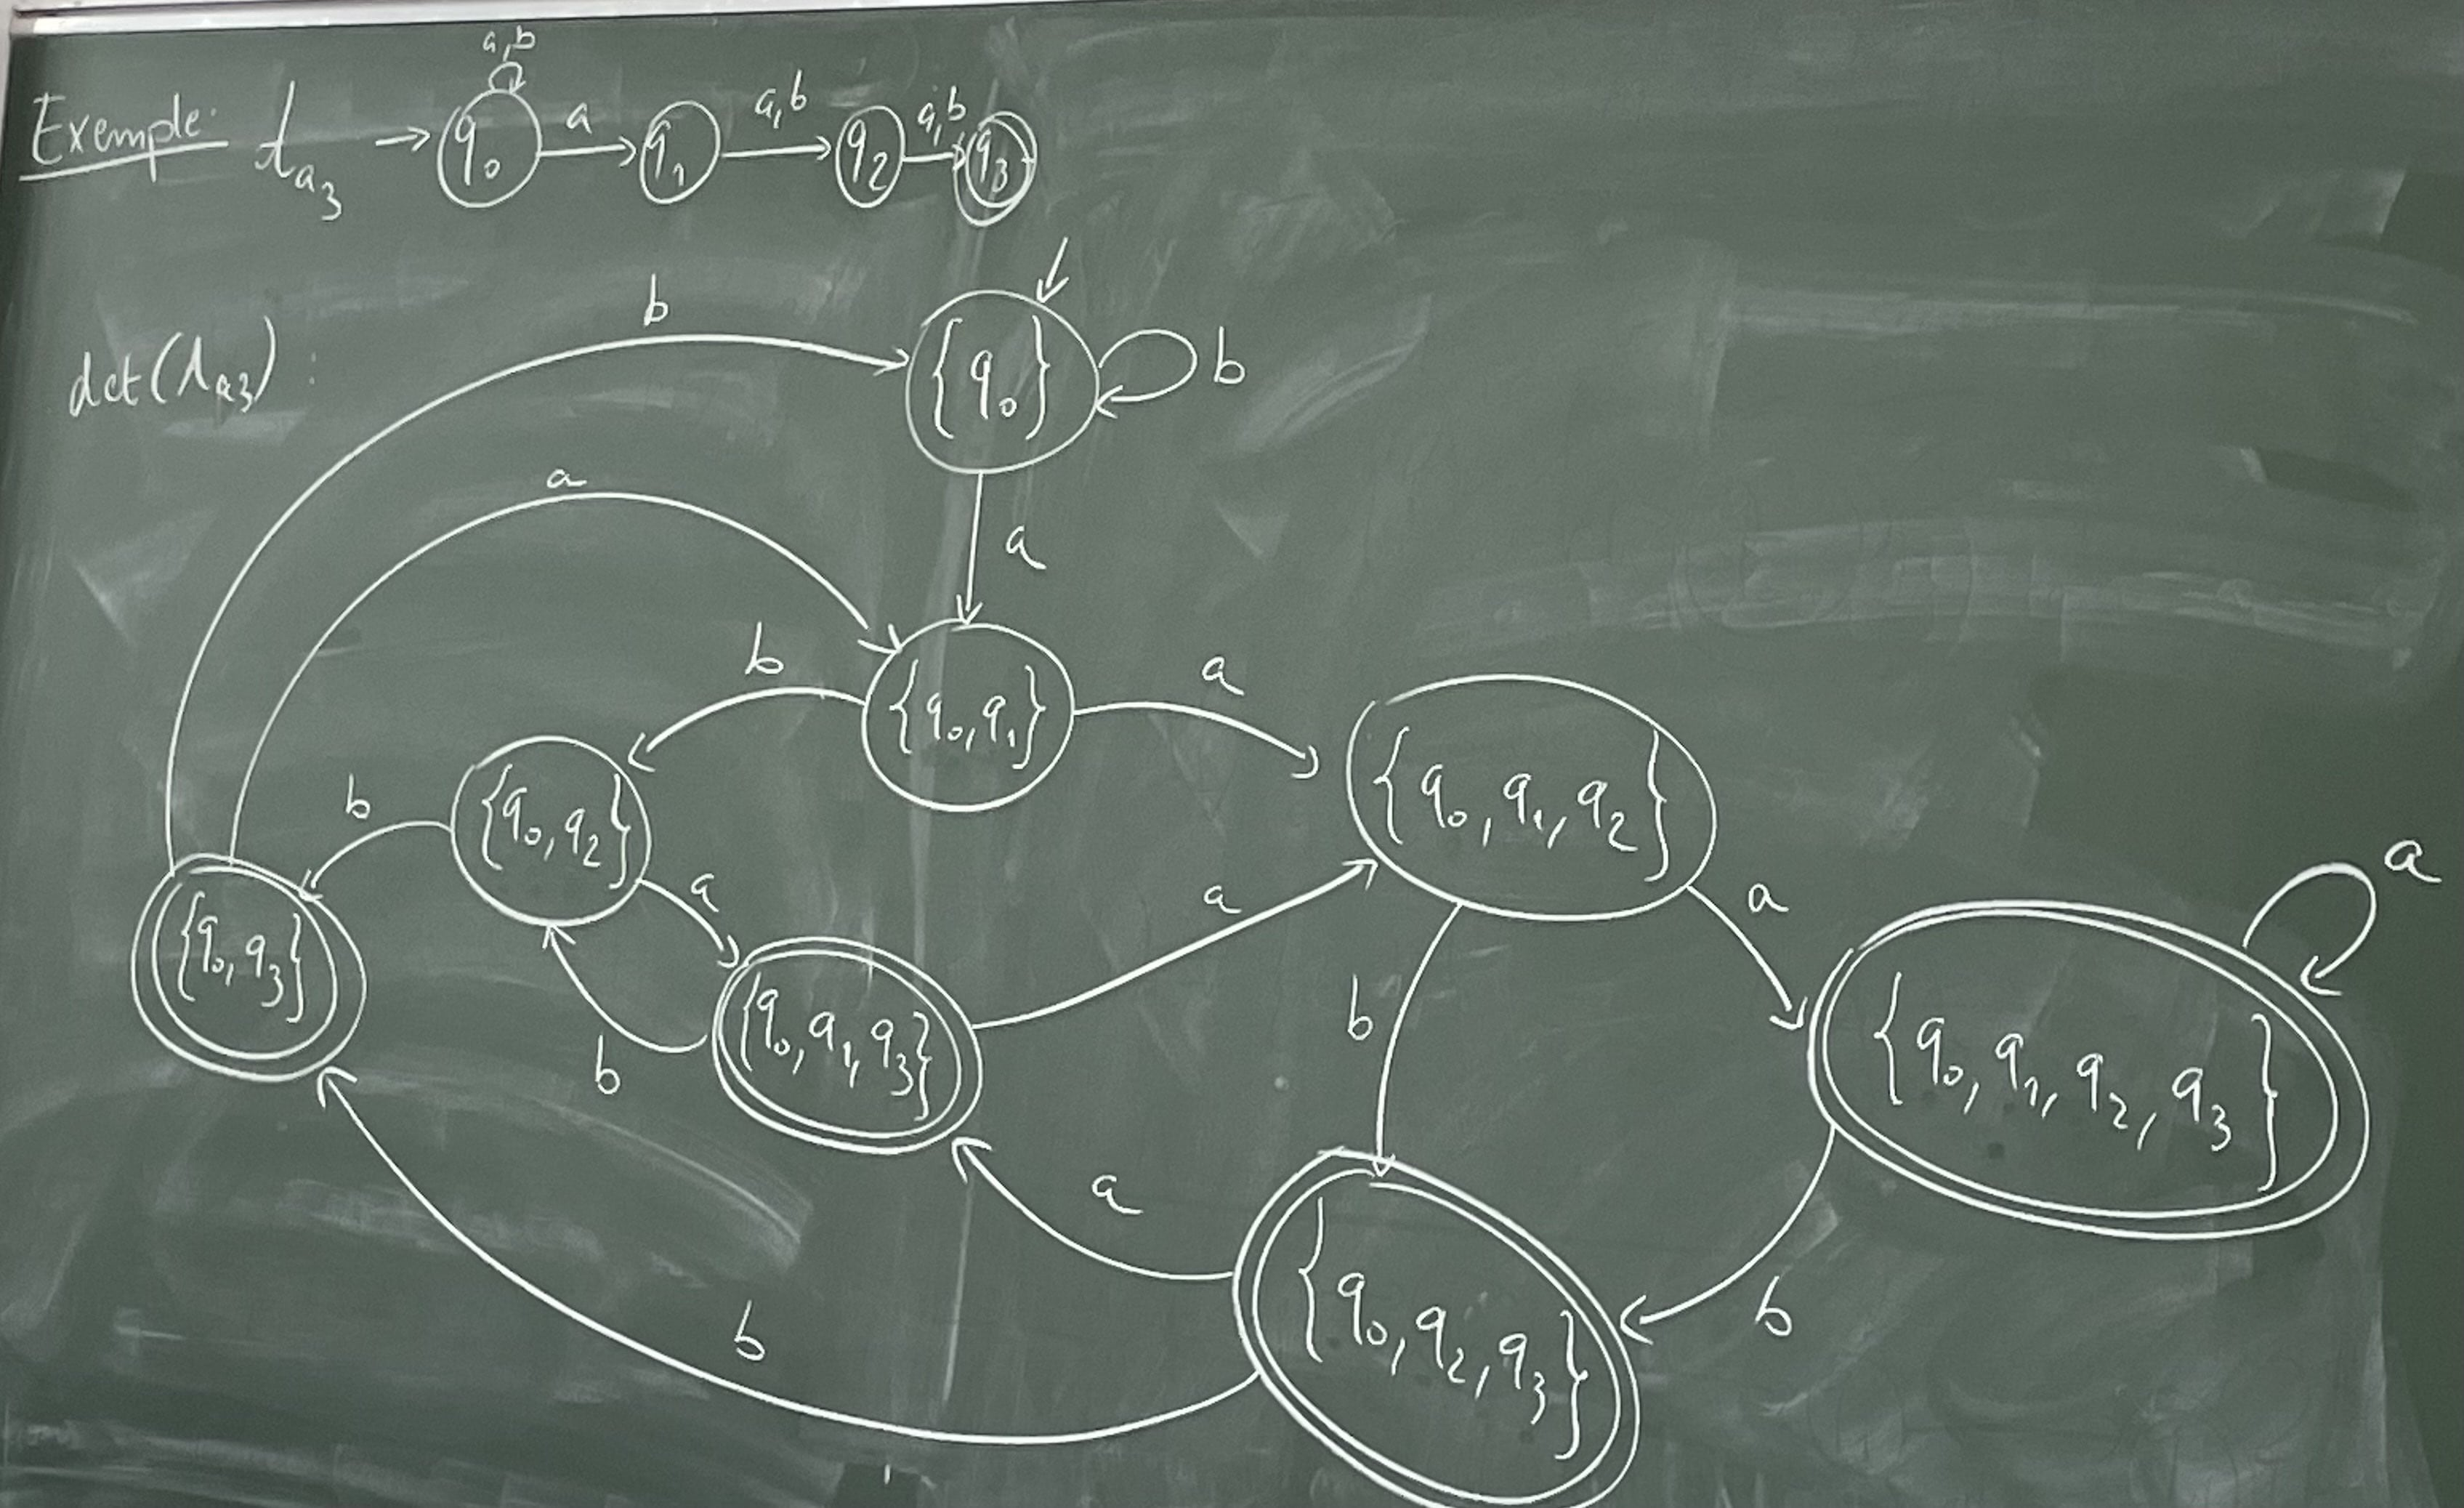
\includegraphics[scale=0.1]{Dessin/Gros_dessin.jpeg}
    \end{example}
    
    \begin{theorem}{}{}
        Soit $\bcA_N = \p{Q_N, \Sigma, q_0, F_n, \delta_n}$ un NFA.
        On a $\bcL\p{\bcA_n} = \bcL\p{\det\p{\bcA_n}}$
    \end{theorem}
    
    \begin{nproof}
        Montrons que $\forall v \in \Sigma^\star$ et $r_0 \to r_1 \to \dots \to r_n$ l'unique chemin dans $\det \p{\bsA_n}$ pour $v$ (avec $R_0 = \ens{q_0}$), on a $R_n = \ens{q \in Q_n \enstq \exists q_0 \lima{v}{\bsA_n^\star} q}$.
        
        Par récurrence sur $\mod{v}$ :
        %
        \begin{enumerate}
            \itt si $\mod{v} = 0 : v = \epsilon$ donc $R_0 = \ens{q_0}$, alors c'est bon.
            
            \itt $\mod{v} = n + 1$ : Supposons la propriété vraie pour tout mot de taille $n$ Montrons qu'elle est vraie pour $v$ :
            
            $v = ua$ avec $\mod{u} = n$ et $a \in \Sigma$.
            
            Soit $R_0 \lima{u} {}^\star R_n \lima{a}{} R_n+1$ dans $ \det{\bsA_n}$.
            
            Par hypothèse de récurrence, $R_n = \ens{q \in Q_n \enstq \exists q_0 \lima{u}{\bsA_n^\star} q}$
            
            Par définition de $\delta_\bsD$ :
            $R_{n+1} = \delta_\bsD \p{R_n, a} = \bigcup_{q \in R_n} \delta_n \p{q, a} = \ens{q' \ in Q_n \enstq \exists \lima{v}{\bsA_n}^\star q'}$
            
            \itt On a fait toutes les positions des chemins : $q_0 \lima{u}{\bsA_n}^\star q'$
        
        
        
            Par définition de $F_d$
            
            \begin{align*}
                v \in \bcL\p{\det{A_n}} &&\iff&& \ens{q_0} \lima{v^\star} R_n &&\text{avec} \ R_n \cap F_n \neq \emptyset\\
                &&\iff&& \exists q_0 \lima{v}^\star_{\bcA_n} q &&\text{avec} q \in F_n
            \end{align*}
            
        \end{enumerate}
    \end{nproof}
    
    \begin{corollary}{}{}
        Soit $L \subseteq \Sigma^\star$ un langage : L est reconnaissable par un DFA si et seulement si L est reconnaissable par un NFA.
    \end{corollary}
    
    \begin{nproof}
        ($\Leftarrow$<=) Si $L = \bsL \p{\bsA_n}$ avec $\bsA_n$ DFA alors $L = \bsL \p{\bsA_\bsD}$ avec $\bsA_\bsD = det \p{\bsA_n}$
        ($\rightarrow$=>) Si $\bsA_\bsD = \p{Q, \Sigma, q_0, F, \delta_\bsD}$ un DFA tq $L = \bsL \p{\bsA_\bsD}$
        Alors$\bsA_n = \p{Q, \Sigma, q_0, F, \delta_n}$ avec $\delta_n \p{q, a} = \ens{\delta_\bsD \p{q, a}}$ pour tout $q \in \alpha, a \in \Sigma$ vérifie $L \in \bsL \p{\bsA_n}$
    \end{nproof}
    
    On va maintenant montrer comment supprimer les $\epsilon$-transitions.
    
    \begin{definition}{$\epsilon$-fermeture}{}
        Soit $\bsA = \ens{Q, \Sigma, q_0, F, \delta}$ un $\epsilon$-NFA. 
        Soit $q\in Q $ %une ligne
        
        on appelle $\varepsilon$-fermeture de q l'ensemble: 
        
        %remy a supprimer la formule
        
    \end{definition}
    \begin{notation}
        Si $Q' \subseteq \text{  , } E(Q') = \bigcup E(q) $ 
        
    \end{notation}
    
    %manque 1 definition, 1 notation, 1 theoreme, 1 corrolaire, 1 definition 
    
    \subsection{Theoreme de Kleeme}
    
    \begin{theorem}{de Kleeme}{}
    Soit $\Sigma$ un alphabet 
    
    
    $Rcc_\Sigma = Reg_\Sigma$
    
    %il manque un gros paragraphe 
    
    \end{theorem}
    \begin{definition}{automates de Thomposon}{}
        
    \end{definition}
    
    \begin{nproof}{Par induction}
        plein de petite dessin par millier 
        
    \end{nproof}
    
    On remarquera que dans les automates de \textsc{Thompson}, on a souvent la situation suivante :
    %
    \begin{tikzpicture}
        
    \end{tikzpicture}
    %
    En réalité, les \guill{vrais} états initiaux sont $q_{i_1}, \dots, q_{i_n}$ mais notre définitions des automates impose d'avoir un seul état initial. Dans la définitions des NFA, on peut en fait autoriser un ensemble $I \subseteq Q$ d'états initiaux au lieu d'un unique $q_0$. Dans ce cas, pour l'automate des parties (algorithme pour déterminer un NFA), il faut choisir $I$ à la place de $\ens{q_0}$ pour l'état initial.
    
    \begin{theorem}{}{}
        Soient \hg{$\Sigma$ un alphabet} et \hg{$r$ une expression régulière} sur $\Sigma$. On a :
        %
        \[ \hg{\bcL\p{\th r} = \bcL\p{r}}\]
    \end{theorem}
    
    \begin{nproof}
        Soient $\Sigma$ un alphabet et $r$ une expression régulière sur $\Sigma$. On procède par induction structurelle sur $r$. Traitons d'abord les cas de base :
        %
        \begin{enumerate}
            \itt Si $r = \emptyset$, on a $\th r = \th \emptyset = $ dessin.
            
            Dans ce cas, $\bcL\p{\th r}\bcL\p{\th \emptyset} = \emptyset = \bcL\p{\emptyset} = \bcL\p{r}$.
            
            \itt Si $r = \epsilon$, on a $\th r = \th \epsilon = $ dessin.
            
            Dans ce cas, $\bcL\p{\th r} = \bcL \p{\th \epsilon} = \ens{\epsilon} = \bcL\p{\epsilon} = \bcL\p{r}$
            
            \itt Si $r = a$, on a $\th r = \th a = $ dessin.
            
            Dans ce cas, $\bcL\p{\th r} = \bcL \p{\th a} = \ens{a} = \bcL\p{a} = \bcL\p{r}$
        \end{enumerate}
        %
        Pour l'induction, on considère $r_1$ et $r_2$ deux expressions régulières telles que :
        %
        \[ \bcL\p{\th r_1} = \bcL\p{r_1} \qquad\et\qquad \bcL\p{\th r_2} = \bcL\p{r_2} \]
        %
        On pose $A_1 = \th r_1$ et $A_2 = \th r_2$. Traitons alors les différentes règles d'induction, en considérant un $r$ obtenu à partir de $r_1$ et $r_2$. On pose directement $A = \th r$. On a :
        %
        \begin{enumerate}
            \itt Si $r = r_1r_2$, alors :
            %
            \[ A :\quad \to q_1 \lima{\epsilon} q_i^1 A_1 q_f^1 \lima{\epsilon} q_i^2 A_2 q_f^2 \lima{\epsilon} q_f\]
            %
            Soit $v \in \bcL\p{r_1r_2}$, alors il existe $v_1 \in \bcL\p{r_1}$ et $v_2 \in \bcL\p{r_2}$. Par hypothèse, on a donc $v_1 \in \bcL\p{A_1}$ et $v_2 \in \bcL\p{A_2}$.
            
            Puisque $v_1 \in \bcL\p{A_1}$, il existe un chemin $q_i^1 \lima{v_1}_{A_1}^\star q_f^1$.
            
            De même, $v_2 \in \bcL\p{A_2}$, il existe un chemin $q_i^2 \lima{v_2}_{A_2}^\star q_f^2$.
            
            Donc :
            %
            \[ q_i \lima{\epsilon} q_i^1 \lima{v_1}{}_A^\star q_f^1 \lima{\epsilon}  q_i^2 \lima{v_2}{}_A^\star q_f^2 \lima{\epsilon}  q_f\]
            %
            Donc $\epsilon v_1 \epsilon v_2 \epsilon \in \bsL \p{A}$
        (car $\epsilon v_1 \epsilon v_2 \epsilon = v_1 v_2 = v$)
        ainsi $\bsL\p{r_1r_2} \subseteq \bsL(A)$ 
            
        
        Réciproquement, si $v\in \bsL(\bcA)$, forcément le chemin acceptant $v$ dans $\bcA$ est de la forme précédente, donc $v= \epsilon v_1 \epsilon v_2  \epsilon $
        
        
        Donc $v = v_1v_2$ avec $v_1 \in \bcL\p{A_1} = \bcL\p{r_1}$ et $v_2 \in \bcL\p{A_2} = \bcL\p{r_2}$ d'où $v \in \bcL\p{r_1r_2}$, ainsi $\bcL\p{A} \subseteq \bcL\p{r_1r_2} = \bcL\p{r}$.
        
            \itt Si $r = r_1 \vert r_2$, alors :
            
            \textcolor{magenta}{DESSIN}
            
            Soit $v \in \bcL\p{r_1 \vert r_2}$. Par hypothèse d'induction, on a $v \in \bcL\p{A_1}$ donc $q_i^1 \lima{v}_{A_1}^\star q_f^1$. Par construction, 
            %
            \[ q_i \lima{\epsilon} q_i^1 \lima{v}_A^\star q_1^f \lima{\epsilon} q_f\]
            %
            accepte $v$ dans $A$, donc $v \in \bcL\p{A}$, d'où $\bcl\p{r_1 \vert r_2} \subseteq \bcL\p{\bcA} = \bcL\p{\th r}$.
            
            Réciproquement, si $v \in \bcL\p{A}$, alors son chemin acceptant est de la forme :
            %
            \[ q_i \lima{\epsilon} q_i^1 \lima{v}_{A}^\star q_f^1 \lima{\epsilon} q_f \qquad\ou\qquad TODO\]
            %
            Donc $v \in \bcL\p{A_1}$ ou $v \in \bcL\p{A_2}$. Par hyptohèse d'induction, $v \in \bcL\p{r_1} \cup \bcL\p{r_2} = \bcL\p{r_1 \vert r_2}$.
            
            \itt Si $r = r_1^\star$, alors :
            %
            \textcolor{magenta}{\Huge{DESSIN}}
            %
            Soit $v \in \bcL\p{r_1^\star} = \bcL\p{r_1}^\star$. Il existe un entier $m \in \bcN$ tel que $v = v_1 \dots v_m$ avec $v_i \in \bcL\p{r_1}$ pour $i \in \iint{1, m}$.
            
            Montrons par récurrence sur m que $v \in \bsL \p{A}$ :
            \begin{enumerate}
                \ithand Si $m = 0$, alors $v = \epsilon \in \bsL \p{A}$ car $q_i \lima{\epsilon} q_i^1 \lima{\epsilon} q_f^1 \lima{\epsilon}  q_f$
                    
                \ithand Si $m \geq 1$, alors par hypothèse de récurrence, $v_1\cdots v_{n+1} \in \bcL\p{A}$. Donc :
                %
                \[ q_i \lima{\epsilon} q_i^1 \lima{v_1\dots v_{n-1}}_A^\star q_f^1 \lima{\epsilon} q_f\]
                %
                Or $v_m \in \bcL\p{r_1} = \bcL\p{A_1}$ soit l'hypothèse de récurrence. Ainsi $q_i^1 \lima{v_m}_{A_1}^\star q_f^1$.
            \end{enumerate}
                
            Donc $v$ est accepté dans $A$ par:    
            %
            \[ q_i \lima{\epsilon} q_i^1 \lima{v_1 \dots v_{m-1}}_A^\star q_f^1 \lima{\epsilon} q_i^1 \lima{v_m}_A^\star q_f^1 \lima{\epsilon} q_f \]
            %
            Donc $v \in \bcL\p{A}$. Réciproquement, soient $v \in \bcL\p{A}$ et $q_i \lima{v}_A^\star q_f$ acceptant $v$.
            %
            \begin{enumerate}
                \ithand Si $q_i \lima{\epsilon} q_i^1 \lima{\epsilon} q_f^1 \lima{\epsilon} q_f$, alors 
                
                \ithand 
                
                \ithand sinon, on peut toujours se ramener à un chemin n'ayant pas de morceau de la forme :
                %
                \[ q_i \lima{\epsilon} q_i^1 \lima{v_1}_{A_1}^\star q_f^1 \lima{\epsilon} q_i^1 \lima{v_2}_{A_1}^\star \lima{\epsilon} q_i^1 \lima \dots \lima{v_m}ç{A_1}^\star q_f^1 \lima{\epsilon} q_f\]
                %
                Donc $v =v_1 \dots v_m$ avec $v_i \in \bcL\p{A_1} = \bcL\p{r_1}$ pour $i \in \iint{1, m}$, donc $v \in \bcL\p{r_1^\star}$.
             \end{enumerate}
        \end{enumerate}
    \end{nproof}
    
    On remarquera que cette preuve est constructive. Elle fournit donc un algorithme qui, à partir d'une expression régulière $r$, fournit un automate reconnaissant $\bcL\p{r}$. L'automate de \textsc{Thompson} doit son nom à l'informaticien \textsc{Ken Thompson} qui a créé l'outil \texttt{grep}, reposant sur la construction des automates (de \textsc{Thompson}). 
    
    On remarquera par ailleurs que 'l'on vient de montrer que $\mathrm{Reg}_\Sigma \subset \mathrm{Rec}_\Sigma$. La section suivante propose une autre démonstration (elle aussi constructive) de cette inclusion.
    
    \subsubsection{Algorithme de Berry-Sethi, automate de Glushkov}
        
    \begin{definition}{Langage local}{}
        Soit $\Sigma$ un alphabet, et $L \subset \Sigma^\star$ un langage. On note :
        %
        \begin{enumerate}
            \itast $\First\p{L} = \ens{a \in \Sigma \enstq \ens{a}\Sigma^\star \cap L \neq \emptyset}$
            
            \itast $\Last\p{L} = \ens{a \in \Sigma \enstq \Sigma^\star\ens{a} \cap L \neq \emptyset}$
            
            \itast FACTS
            
            \itast NFACTS
        \end{enumerate}
    \end{definition}
    
    \begin{example}
            exemple triviale 
            
            
            
            Soit $v \in (First(L1)\Sigma $ %remy ecrit %LOL NON TA CRU
            
            
    \end{example}
    
    \begin{definition}{automate de Glushkov}{}
        Soit $\Sigma$ un alphabet et $L \subset \Sigma^\star$ un langage local. On appelle \hg{automate de \textsc{Glushkov}} de $L$ l'automate $\Loc{L} = \p{Q_L, \Sigma, q_0, F_L, \delta_L}$ tel que :
        %
        \begin{enumerate}
            \itast $Q_L = \ens{q_0} \cup \ens{q_a \enstq a \in \Sigma}$
            
            \itast $F_L = \ens{q_a \enstq a \in \Last{L}} $
        \end{enumerate}
        
        
    \end{definition}
    
    \begin{theorem}
        Soit $\Sigma$ un alphabet et $L \subseteq \Sigma^\star$ un langage local. $L = \bcL(Loc(L))$
    \end{theorem}
    \begin{nproof}
        L $\subset \bsL(Loc(L))$
        \begin{enumerate}
            \itt \Huge{blablablablbalbal}
        \end{enumerate}
    \end{nproof}
    
    \begin{definition}{Expression linéaire}{}
        Soit \hg{$\Sigma$} un \hg{alphabet}. Une \hg{expression régulière} sur $\Sigma$ est dite \hg{linéaire} lorsque \hg{tout symbole de $\Sigma$ y apparaît au plus une fois}.
    \end{definition}
    
    On a les exemples ci-dessous :
    %
    \begin{example}{}{}
        Considérons l'alphabet $\Sigma$ tel que $\ens{a, b, c} \in \Sigma$.
        \begin{enumerate}
            \itt \hg{$a^\star bc^\star$} est une expression régulière.
            
            \itt \hg{$ba^\star bc^\star b$} n'est \hg{pas} une expression régulière.
        \end{enumerate}
    \end{example}
    
    Montrons d'abord le lemme suivant :
    %
    \begin{lemma}{}{}
        Soient \hg{$\Sigma_1$} et \hg{$\Sigma_2$} deux \hg{alphabets} tels que \hg{$\Sigma_1 \cap \Sigma_2 \neq \emptyset$}, ainsi que \hg{$\bcL_1$} et \hg{$\bcL_2$} deux \hg{langages locaux}, respectivement \hg{sur $\Sigma_1$} et \hg{sur $\Sigma_2$}. Dans ce cas :
        %
        \begin{enumerate}
            \itast \hg{$\bcL_1 \cap \bcL_2$} est un \hg{langage local sur $\Sigma_1 \cap \Sigma_2$} ;

            \itast \hg{$\bcL_1 \cup \bcL_2$} est un \hg{langage local sur $\Sigma_1 \cup \Sigma_2$} ;
            
            \itast \hg{$\bcL_1 \cdot \bcL_2$} est un \hg{langage local sur $\Sigma_1 \cup \Sigma_2$} ;
            
            \itast \hg{$\bcL_1^\star$} est un \hg{langage local}.
        \end{enumerate}
    \end{lemma}
    
    \begin{nproof}
        Soient $\Sigma_1$ et $\Sigma_2$ deux alphabets tels que $\Sigma_1 \cap \Sigma_2 \neq \emptyset$, $\bcL_1$ un langage local sur $\Sigma_1$ et $\bcL_2$ un langage local sur $\Sigma_2$.
        
        On note pour \(i\in \ens{1, 2}\) : \(La_i =\) Last(\(L_i\)), \(Fi_i =\) First(\(L_i\)), \(Fa_i =\) Fact(\(L_i\)), \(NFa_i\) = NFact(\(L_i\))

        \begin{psse}
            \item Si \(v \in \left(\bcL_1\cap\bcL_1\right)\backslash\ens{\varepsilon}\) alors \(v = a_i \hdots a_n\) avec \(a_1 \in Fi_1 \cap Fi_2\) et \(a_n \in \bcL a_1 \cap \bcL a_2\) et \(\forall i, a_i a_{i+1} \in Fa_1 \cap Fa_2\)

            Et réciproquement, tout mot vérifiant ces trois propriétés est dans les langages car ils sont locaux. donc en posant \(Fi = Fi_1 \cap Fi_2\), \(La = La_1 \cap La_2\) et ainsi de suite on a go 
            \[ \left(\bcL_1\cap \bcL_2 \right) \backslash \ens{\varepsilon} = \left(Fi\Sigma^{\alpha} \cap \Sigma^{\alpha} \bcL a\right) \backslash \Sigma^{\alpha} NFa \Sigma^*\]

            On vérifie facilement que les nouveaux ensembles sont les caractéristiques de \(\bcL=\bcl_1\cup\bcL_2\)
            
            Donc $L \backslash \ens{\varepsilon} \subseteq \quad (F_i \Sigma^* \cap \Sigma^* $

            \item Réciproquement  si \(v\in \bcL\backslash\ens{\varepsilon}\), alors :
            %
            $v = a_1\dots a_n$ et si $a_1 \in F_{i_1}$, donc $a_1 \in \Sigma_1$.
            
            Donc $a_1a_2 \in F_{a_1}$ (car $\Sigma_1 \cap \Sigma_2 \neq \emptyset$).
            
            Donc $a_2 \in \Sigma_1$, \dots
            
            On montre de proche en proche (car $\Sigma_1 \cap \Sigma_2 \neq \emptyset$) que $v \in \Sigma_1^\star$ et que pour tout $i \in \iint{1, n-1}$, $a_ia_{i+1} \in F_{a_1}$. De plus, $a_1 \in \bcL_\epsilon  = \bcL_{a_1} \cup \bcL_{a_2}$.
            
            Or $a_n \in \Sigma_1$ donc $a_n \in \bcL_{a_1}$. Donc $v \in \bcL_1$ (car $\bcL_1$ est local) d'où $v \in \bcL$.
            
            Si $a_1 \in F_{i_2}$, on montre de manière similaire que $v \in \bcL_2$, donc que $v \in \bcL$. Au final, $\bcL' \backslash \ens{\epsilon} \subseteq \bcL \backslash \ens{\epsilon}$, et donc $\bcL$ est un langage local.
            
            \item Notons $\bcL = \bcL_1 \cdot \bcL_2$. Les ensembles caractéristiques de $\bcL$ sont $\bcF_i = \left\lbrace \begin{array}{ll}
                \bcF_{i_1} &\text{si} \ \epsilon \not\in \bcL_1  \\
                \bcF_{i_1} \cup \bcF_{i_2} &\text{sinon} 
            \end{array}\right.$ et $\bcL_a = \left\lbrace \begin{array}{ll}
                \bcL_{a_2} &\text{si} \ \epsilon \not\in \bcL_2  \\
                \bcL_{a_1} \cup F_{a_2} &\text{sinon} 
            \end{array}\right.$.
            
            On a $\bcF_a = \bcF_{a_1} \cup \bcF_{a_2} \cup \p{\bcL_{a_1} \cdot \bcF_{i_2}}$ donc on a bien $\bcL \backslash \ens{\epsilon} \subseteq \underbrace{\p{\bcF_i \Sigma^\star \cap \Sigma^\star L_a} \backslash \Sigma^\star NF_\alpha \Sigma^\star}_{\bcL'}$.
            
            Soit $v \in \bcL' \backslash \ens{\epsilon}$. On a $v = a_1 \dots a_n$, et :
            %
            Si $a_1 \in \bcF_{i_2}$, alors $\epsilon \in \bcL_1$. Comme $\Sigma_1 \cap \Sigma_2 \neq \emptyset$, on montre, comme dans le cas précédent de proche en proche, que $v \in \Sigma_2^\star$ et que pour tout $i \in \iint{1, n-1}$ on a $a_ia_{i+1} \in \bcF_{a_2}$ et $a_n \in \bcL_{a_2}$. Ainsi, $v \in \bcL_2$ car le langage est local.
            
            Or $\epsilon \in \bcL_1$ donc $v \in \bcL = \bcL_1 \cdot \bcL_2$.
            
            Si $a_1 \in F_{i_1}$, soit $a_1 \dots a_p$ le plus long préfixe de $v$ dans $\Sigma_1^\star$. On a:
            \begin{enumerate}
                \itt $a_1$ \in $\bcF_{i_1}$ ;
                
                \itt $\forall i \ in [|1, p-1|] a_i a_{i+1} \in F_{a1} $%va y 
                
                \itt montrons que $a_p \in \bcL_{a_1}$ : si $p = n$, on a $a_p \in \bcL_a \cap \Sigma_1 = \bcL_{a_1}$ et forcément $\epsilon \in $ ....

                Donc $v= \underbrace{a_1 \dots a_p}_{\in \bcL_1} \underbrace{a_{a+1} \dots a_n}_{\in \bcL_2} \in L_1 \cdot L_2$, d'où $L_1\cdot L_2$ est local.
                
            \end{enumerate}     
            
            \item Notons $\bcL = \bcL_1^\star$. On a $\bcF_i = \bcF_{i_1}$, $\bcL_a = \bcL_{a_1}$ et $\bcF_a = \bcF_{a_1} \cup \p{\bcL_{a_1} \cdot \bcF_{i_1}}$.
                
            On a bien $\bcL \backslash \ens{\epsilon} \subseteq L'$.
                
                Soit $v \in L' \backslash \ens{epsilon} $
                %il effacer le tableau

        \end{psse}
    \end{nproof}
    
    
    \begin{property}{}{}
        Soient \hg{$\Sigma$} un \hg{alphabet} et \hg{$r$} une \hg{expression régulière} sur $\Sigma$.
        %
        \[ \hg{\text{Si} \ r \ \text{est linéaire, alors} \ \bcL\p{r} \ \text{est local.}} \]
    \end{property}
    
    \begin{nproof}
        Soient $\Sigma$ un alphabet et $r$ une expression régulière sur $\Sigma$.
        %
        \begin{enumerate}
            \itt Si \(r = \emptyset : \bcL(r) = \emptyset\) est bien local
            \itt Si \(r= \epsilon : \bcL(\epsilon) = \ens{\epsilon}\) est bien local
            \itt Si \(r=a, \bcL(a) = \ens{a}\) est bien local

            \itt Si \(r = r_1 \mid r_2\) avec par hypothèse d'induction \(r_1\) et \(r_2\) locaux, comme \(r\) est linéaire on a que \(r_1\) et \(r_2\) sont distincts donc par lemme(2) \(\bcL(r) = \bcL(r_1)\cup\bcL(r_2)\)

            \itt Si \(r = r_1 \cdot r_2\) par hypothèse d'induction \(\bcL(r_1)\) et \(\bcL(r_2)\) sont locaux et par linéarité de \(r\) les deux alphabets sont distincts donc \(\bcl(r_1\cdot r_2) = \bcL(r_1) \cdot \bcL(r_2)\) par lemme (3) donc le langage est local.

            \itt Si \(r = r_1^*\) par hypothèse d'induction \(\bcL(r_1)\) est local et par lemme (4) \(\bcL(r_1^*) = \bcL(r_1)^*\) est local.
        \end{enumerate}
    \end{nproof}
    
    \begin{definition}{Linéarisation}
        Si r est une expression régulière sur $\Sigma$ on peut le transformer en une 
        expression régulière linéaire linéaire sur $\Sigma'$ avec le processus suivant
        \begin{enumerate}
            \itast On initialise \(\Sigma' = \emptyset\)
            \itast On lit \(r\) de gauche à droite 
            \itast Si \(a\in\Sigma\) est la \(i\)-ème lettre de \(r\) on la remplace par une lettre notée \(a_i\) qui ajoute \(a\) dans \(\Sigma'\)
        \end{enumerate}
    \end{definition}
    
    \begin{example}{}{}
        Considérons l'expression régulière \hg{$r$} sur l'alphabet $\hg{\Sigma = \ens{a, b}}$ suivante :
        %
        \[ \hg{r = a\p{ab}^\star \vert b^\star a}\]
        %
        On \hg{linéarise $r$ en l'expression $r'$} sur $\hg{\Sigma' = \ens{a_1a_2b_3b_4a_5}}$ :
        %
        \[ \hg{r' = a_1\p{a_2b_3}^\star \vert b^4a_5 } \]
    \end{example}
    
    \begin{form}{Algorithme de Berry-Sethi}{}
        Soient \hg{$\Sigma$} un \hg{alphabet} et $r$ une \hg{expression régulière} sur $\Sigma$. L'\hg{algorithme de \textsc{Berry-Sethi}} consiste à :
        
        \begin{psse}
            \item \hg{linéariser $r$} en \hg{$r'$} ;
            
            \item \hg{calculer $\First{\bcL\p{r'}}$}, \hg{$\Last{\bcL\p{r'}}$} et \hg{$\Fact{\bcL\p{r'}}$} ;
            
            \item \hg{construire $\bcA = \Loc{\bcL\p{r'}}$} ;
            
            \item \hg{effacer} les \hg{indices des symboles} dans les \hg{transitions de $\bcA$}.
        \end{psse}
    \end{form}
    
    \begin{notation}
        Si \hg{$\bcA = \left( Q,\Sigma',q_0,F,\delta'\right)$} on obtient d'après l'étape \pssenum{iv} : 
        %
        \[ \hg{f\p{\bcA} = \p{Q,\Sigma,q_0,F,\delta}} \qquad\text{où}\qquad \forall \p{q, a_i} \in \mathrm{dom}{\delta'},\qquad \delta\p{q,f(a_i)} = \delta'\p{q,a_i}\]
    \end{notation}
    
    \begin{theorem}{}{}
        Soit $r$ une expression régulière sur $\Sigma$. A la fin de l'algorithme de \textsc{Berry-Sethi}, on obtient un automate $f\p{\bcA}$ tel que $\bcL\p{r} = \bcL\p{f\p{\bcA}}$.
    \end{theorem}
    
    \begin{nproof}
        D'après les résultats précédents, $r'$ est linéaire, donc $\bcL\p{r'}$ est local, doc $\bcA = \Loc\p{\bcL\p{r'}}$ vérifie $\bcL\p{\bcA} = \bcL\p{r'}$, avec $f\p{r'} = r$. Montrons que $\bcL\p{f\p{A}} = \bcL\p{r}$ par double inclusion.

        \begin{enumerate}
            \itt $\boxed{\supseteq}$ Soit $u \in \bcL\p{r}$. Si $u \in \bcL\p{r'}$, alors $\epsilon \in \bcL\p{r'}$, donc $\epsilon \in \bcL\p{\bcA}$. Dès lors, $q_0 \in \bcF$, d'où $\epsilon \in \bcL\p{\bcF\p{A}}$.
            
            Sinon, on a $u = u_1\dots u_n$, et donc il existe $u' \in \bcL\p{r'}$ tel que $u = f\p{u'}$. Ici $u' \in \bcL\p{\bcA}$, donc il existe un chemin dans $\bcA$ : \qquad $q_0 \xrightarrow{u_1'} q_1 \xrightarrow{u_2'} q_2 \dots \xrightarrow{u_n'} q_n \in F$. Ainsi 
            %
            \[ q_0 \xrightarrow{f\p{u_1'}} q_1 \xrightarrow{f\p{u_2'}} q_2 \dots \xrightarrow{f\p{u_n'}} q_n \in F \qquad \text{est un chemin dans} \ f\p{A}\]
            %
            Donc le chemin : \qquad $q_0 \xrightarrow{f\p{u_1}} q_1 \xrightarrow{f\p{u_2}} \dots \xrightarrow{f\p{u_n}} q_n$ est un chemin acceptant $u$ dans $f\p{\bcA}$, donc $u \in \bcL\p{f\p{\bcA}}$.
            
            \itt $\boxed{\subseteq}$ Soit $u \in \bcL\p{f\p{\bcA}}$, si $u = \epsilon$, alors $\epsilon \in \bcL\p{f\p{\bcA}}$, donc $q_0 \in \bcF$, donc $\epsilon \in \bcL\p{\bcA} = \bcL\p{r'}$ d'où $\epsilon \in \bcL\p{r}$.
            
            Sinon, $u = u_1 \dots u_n$, ainsi il existe un chemin dans $f\p{\bcA}$ :
            %
            \[ q_0 \xrightarrow{f\p{u_1}} q_1 \dots \xrightarrow{f\p{u_2}} q_2 \dots \xrightarrow{f\p{u_n}} u_n \in F\]
            %
            Pour $i \in \iint{1, n}$, la transition $q_{i-1} \xrightarrow{f\p{u_i}} q_i$ de $f\p{\bcA}$ correspond à une transition $q_{i-1} \xrightarrow{u_i} q_i$ de $\bcA$ avec $f\p{u_i'} = u_i$, donc :
            %
            \[ q_0 \xrightarrow{f\p{u_1'}} q_1 \xrightarrow{f\p{u_2'}} q_2 \dots \xrightarrow{f\p{u_n'}} q_n \in F\]
            %
            est un chemin acceptant $u' = u_1'\dots u_n'$ dans $\bcA$, donc $u' \in \bcL\p{\bcA} = \bcL\p{r'}$, et ainsi $u = f\p{u'} = \bcL\p{f\p{r'}} = \bcL\p{r}$.
        \end{enumerate}
    \end{nproof}
    
    \begin{example}{}{}
        Reprenons l'expression régulière $r$ sur l'alphabet $\hg{\Sigma = \ens{a, b}}$ précédente ($\hg{r = a\p{ab}^\star \vert b^\star a}$), qu'on avait linéarisée sur $\hg{\Sigma' = \ens{a_1a_2b_3b_4a_5}}$ en :
        %
        \[ \hg{r' = a_1\p{a_2b_3}^\star \vert b^4a_5 } \]
        %
        On obtient alors :
        %
        \begin{enumerate}
            \itt $\hg{\First{\bcL\p{r'}} = \ens{a_1, b_4, a_5}}$ ;
            
            \itt $\hg{\Last{\bcL\p{r'}} = \ens{a_1, b_3, a_5}}$ ;
            
            \itt $\hg{\Fact{\bcL\p{r'}} = \ens{a_1a_2, a_2b_3, b_3a_2, b_4a_5, b_4b_4}}$ ;
        \end{enumerate}
        %
        Ceci permet d'obtenir l'automate de $r$ :
        %
        \begin{center}
            DESSIN
        \end{center}
    \end{example}
    
    On remarque que la construction de Gluskow est donc une alternative à la 
    construction de Thompson. 
    \begin{enumerate}
        \itt L'avantage de la construction de Thompson est qu'elle est plus facile à prouver correcte. 
        
        
        \itt Concernat l'algorithme de Berry-Sethi, sa preuve de correction est moins directe, mais est très facile à faire à la main sur un example, car il a l'avantage: 
        
        \itt    de former un automate avec peu d'états (nombre de lettres dans l'expression de départ
        
        \itt    de fournir un automate sans $\varepsilon$ transition 
    
    \end{enumerate}
    
    
    
    Ces deux constructions sont liées par la propriété suivante :
    
    
    
    \begin{property}{}{}
        Soit $r$ une regex. $rm^\epsilon \p{Th\p{r}} = f\p{\bcL\p{\bcA}}$
    \end{property}
    
    \begin{nproof}
        Admise.
    \end{nproof}
    
    \subsubsection{Algorithme d'élimination des états}
    
    On montre maintenant que $Rec_\Sigma \subseteq Reg_\Sigma$, en présentant l'algorithme de Brzozowski et McCuskey. Cet algorithme repose sur une nouvelle définition d'automate.
    
    \begin{definition}{automate généralisé}{}
        Un automate généralisé est un quintuplet $A = \ens{Q, \Sigma, q_0, F, \delta}$ où
        \begin{enumerate}
            \itt $Q, \Sigma, q_0, F$ sont défini comme avant
            \itt $\delta \subseteq Q \times Reg_\Sigma \times Q$ est une relation de transition de A
        \end{enumerate}
    
    \end{definition}
    On remarque que
    \begin{enumerate}
        \itt  dans un tel automate, on a le droit d'étiqueter une transition par n'importe quelle expression régulière (plutôt que $a \in \Sigma$ ou $\epsilon$).
        \itt Utiliser une relation plutôt qu'une fonction dans la définition de $\delta$ va simplifier un peu la définition de l'algorithme qui va suivre.
    \end{enumerate}

    \begin{definition}{chemin}{}
        Soit $A = \p{Q, \Sigma, q_0, F, \delta}$ un automate généralisé, soit $v \in \Sigma^\star$. $v$ est accepté par $A$ si
        \begin{enumerate}
            \itt $\exists n \in \bcN^\star, \exists \p{v_1, \dots, v_n} \in \p{\Sigma^\star}^n$ tel que
            \begin{enumerate}
                \itt $v = v_1 \dots v_n$
                \itt il existe un chemin$q_0 \lima{r_1}{}_A q_1 \lima{r_2}{}_A \dots \lima{r_n}{}_A q_n \in F$ tel que $\forall i \in \iint{1, n}, v_i \in \bcL\p{r_i}$
            \end{enumerate}
        \end{enumerate}
        
    \end{definition}
    
    \begin{definition}{algorithme d'élimination d'états}{}
        Soit $A = \p{Q, \Sigma, q_0, F, \delta}$ un automate.
        \begin{enumerate}
            \item Créer l'automate généralisé $A' = \p{Q \cup \ens{q_i, q_f}, \Sigma, q_i, \ens{q_f}, \delta'}$ avec $\delta' = \delta \cup\ens{\p{q_i, \epsilon, q_0}} \cup \ens{\p{q, \epsilon, q_f} \enstq q \in F}$
            
            Cet automate $A'$ possède un seul état initial $q_i$ sans transition entrante, et un seul état $q_f$ sans transition sortante.
        
            \item on definis 2 procédure auxiliaires
            \begin{enumerate}
                \itt  élimination des transitions tant qu'il existe deux transitions distinctes $q \lima{r_1}{}_{A'} q'$ et $q \lima{r_2}{}_{A'} q'$ (même $q$ et $q'$, les supprimer, et rajouter $q \lima{r_1 \vert r_2}{} q'$
            
                \itt Elimination d'un état q: pour toutes $p \lima{r_1}{}_{A'} q$ et $q \lima{r_2}{}_{A'} s$ dans $\delta'$
                    \begin{enumerate}
                        \itt ajouter : $\left\lbrace\begin{array}{cl}
                            p \lima{r_1 r^\star r_2}{}_{A'} s &\text{si} \ q \lima{1'}^r q\\ %Le \\ pour sauter la ligne
                            p \lima{r_1 r_2}{}_{A'} & \text{sinon}
                        \end{array}\right.$ 
                        
                        %Ensuite tu met un environnement array : le deuxième crochet {cc} indique qu'on aura deux colonnes centrées. Si je voulais une colonne à gauche puis une colonne centrée je mettrait {lc} et si je voulais centré puis à gauche je mettrait {cl}. merci !!!
                        
                        %Donc ici on met {cl}. Et après le "&", on met la suite
                        
                        %ça en gros ça dit à gauche je vais mettre un bracket left (lbrace) et à droite rien, et le \left / \right aide à adapter la taille
                
                        \itt supprimer $p \lima{r_1}{}_{A'} q$ et $q \lima{r_2}{}_{A'} s$
                        
                        \itt supprimer q 
                    \end{enumerate}
                \end{enumerate}
            
            \item Boucle principale de l'algorithme 
                Pour chaque $q \in \emptyset$ 
                \begin{enumerate}
                    \itt éliminer toutes les transitions possibles
                    \itt éliminer l'état $q$
                \end{enumerate}
            \item Une fois que l'automate est réduit à $\to q_i \lima{r}{} q_f \quad \implies$ renvoyer $r$
        \end{enumerate}
    \end{definition}
    
    On remarque que si $\bcA$ possede plusieurs état initiaux $(I \subseteq Q)$
    
    \begin{theorem}{}{}
        A la fin de l'algorithme, $\bcL\p{A} = \bcL\p{r}$.
    \end{theorem}
    
    \begin{nproof}
        \begin{enumerate}
            \itt L'automate généralisé $A'$ vérifie initialement $\bcL\p{A'} = \bcL\p{A}$
            \itt On montre facilement qu'à chaque étape de l'algorithme, la modification effectuée sur $A'$ ne change pas $\bcL\p{A'}$.
            \begin{enumerate}
                \itt élimination des transitions : pour tout mot $v \in \Sigma^\star$ tq$q \lima{v}{}_{A'}^\star q'$, 
                \begin{enumerate}
                    \itt si ce chemin n'utilise pas $q \lima{r_1}{} q'$ ou $q \lima{r_2}{}q'$, alors ce chemin existe toujours après la modification
                    \itt si ce chemin utilise $q \lima{r_1}{} q'$ ou $q \lima{r_2}{}q'$, alors $v \in \bcL\p{}r_1$ ou $v \in \bcL\p{r_2}$
                    Donc $v \in \bcL\p{r_1 \vert r_2}$
                    Donc après la modification, on peut lire v en prenant $q \lima{r_1 \vert r_2}{} q'$
                    \itt Réciproquement, si $q \lima{v}{}_{A'}^\star q'$, après la modification
                    \begin{enumerate}
                        \itt si on n'utilise pas la nouvelle transition : même chemin avant le motif
                        \itt si on utilise $q \lima{r_1 \vert r_2}{} q'$ alors $v \in \bcL\p{r_1 \vert r_2}$, et qu'on pouvait lire $v$ avant le motif avec $q \lima{r_1}{} q'$ ou $q \lima{r_2}{} q'$
                    \end{enumerate}
                \end{enumerate}
                \itt élimination d'un état q :
                % INSERT IMAGE TABLEAU DE GAUCHE
            \end{enumerate}
            \itt De plus, l'algorithme termine, car le nombre de transition et d'états diminue strictement. Ainsi, à la fin, on a  $A'$ de la forme : $\to q_i \lima{r}{} q_f$ et $\bcL\p{A'} = \bcL\p{r} = \bcL\p{A}$
        \end{enumerate}
    
    \end{nproof}
    
    \begin{corollary}{}{}
        Soit $\Sigma$ un alphabet 
        $Rec_\Sigma \subseteq Reg_\Sigma$
    \end{corollary}
    
    \begin{example}{detaille de l'algo }{}
        %j'ai pris des photo de l'exemple 
        %\begin{enumerate}
            %\itt enumeration de $q_0$ : %sous shéma
            %\itt nnouvelles transitions : %sous shéma
            %On obtient : %sous-shéma
        %\end{enumerate}
        
        dessin:
        
        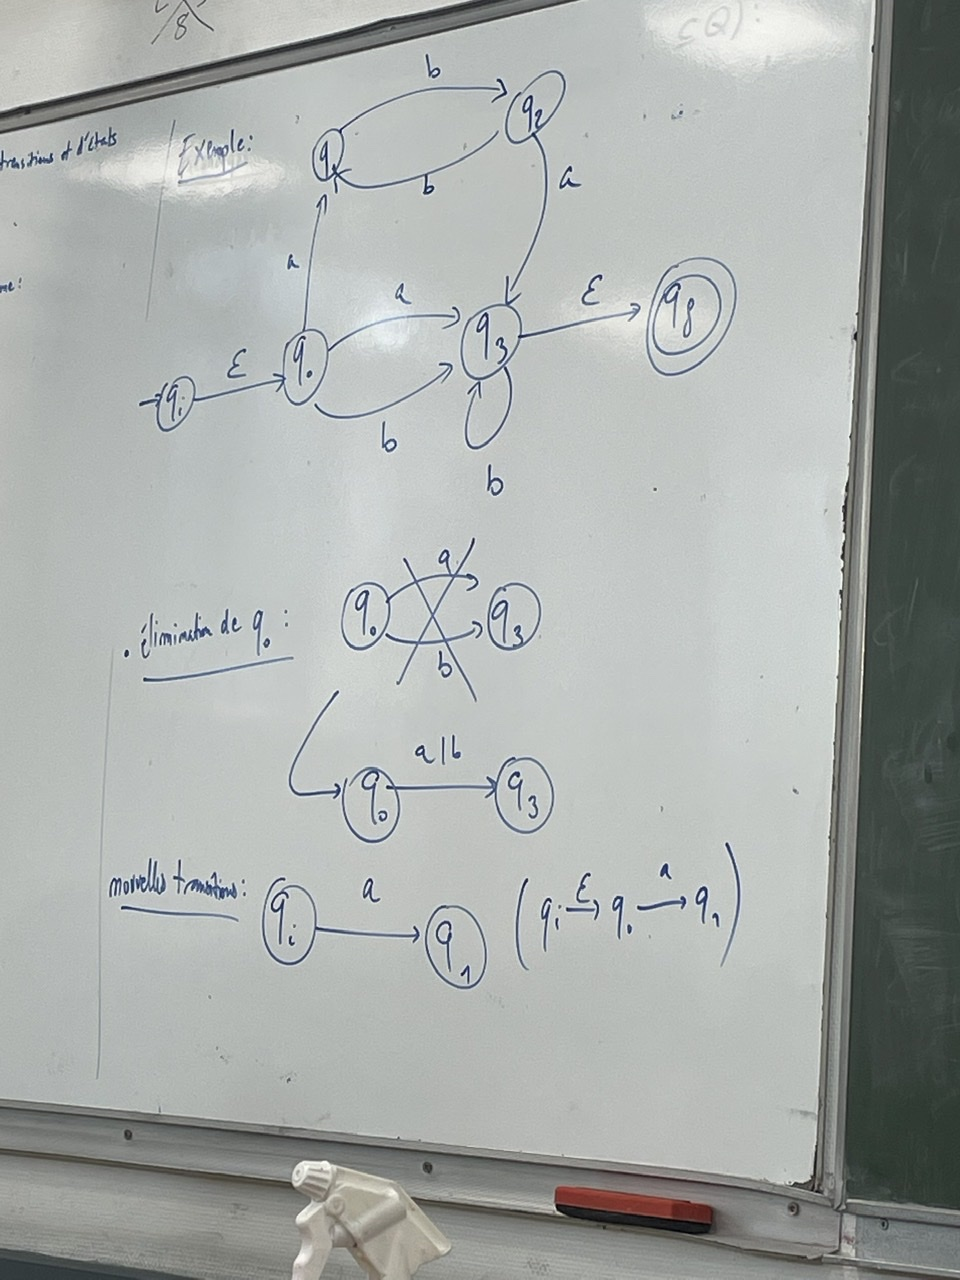
\includegraphics[scale=0.2]{Dessin/Tableau1.jpeg}%giga compresser 
        \vspace{2cm}
        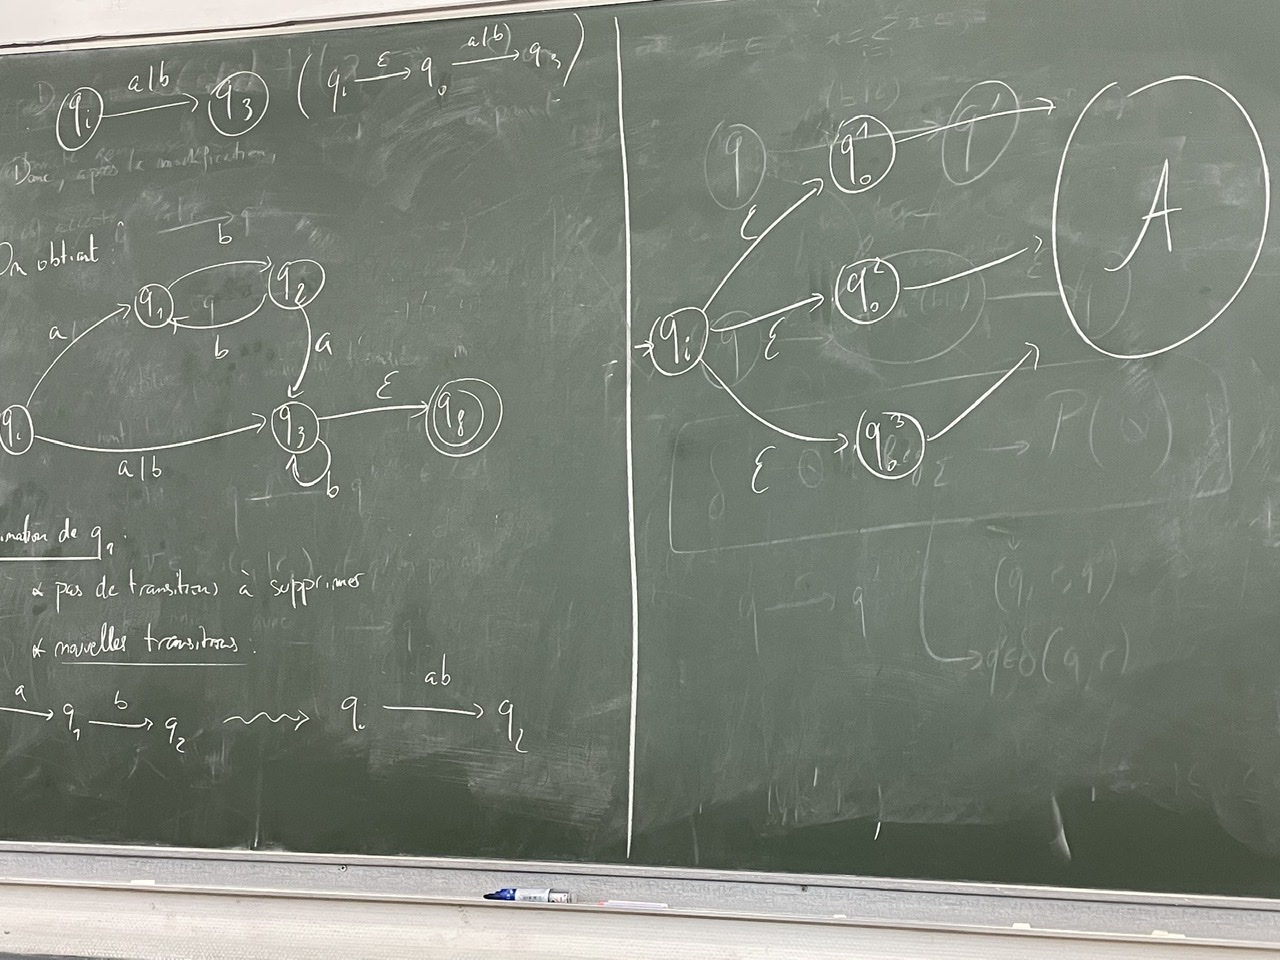
\includegraphics[scale=0.2]{Dessin/Tableau2.jpeg}
        %vive le premium qui donne 4min de temps de compilation 
        \vspace{2cm}
        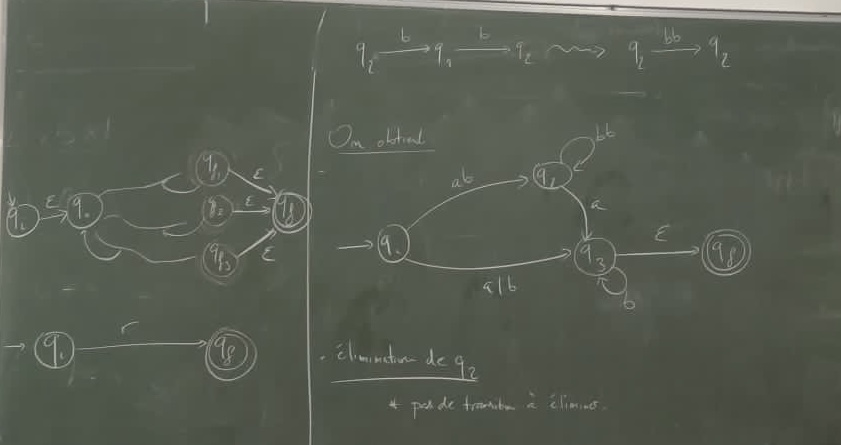
\includegraphics[scale=0.2]{Dessin/Tableau3.jpeg}
        \vspace{2cm}
        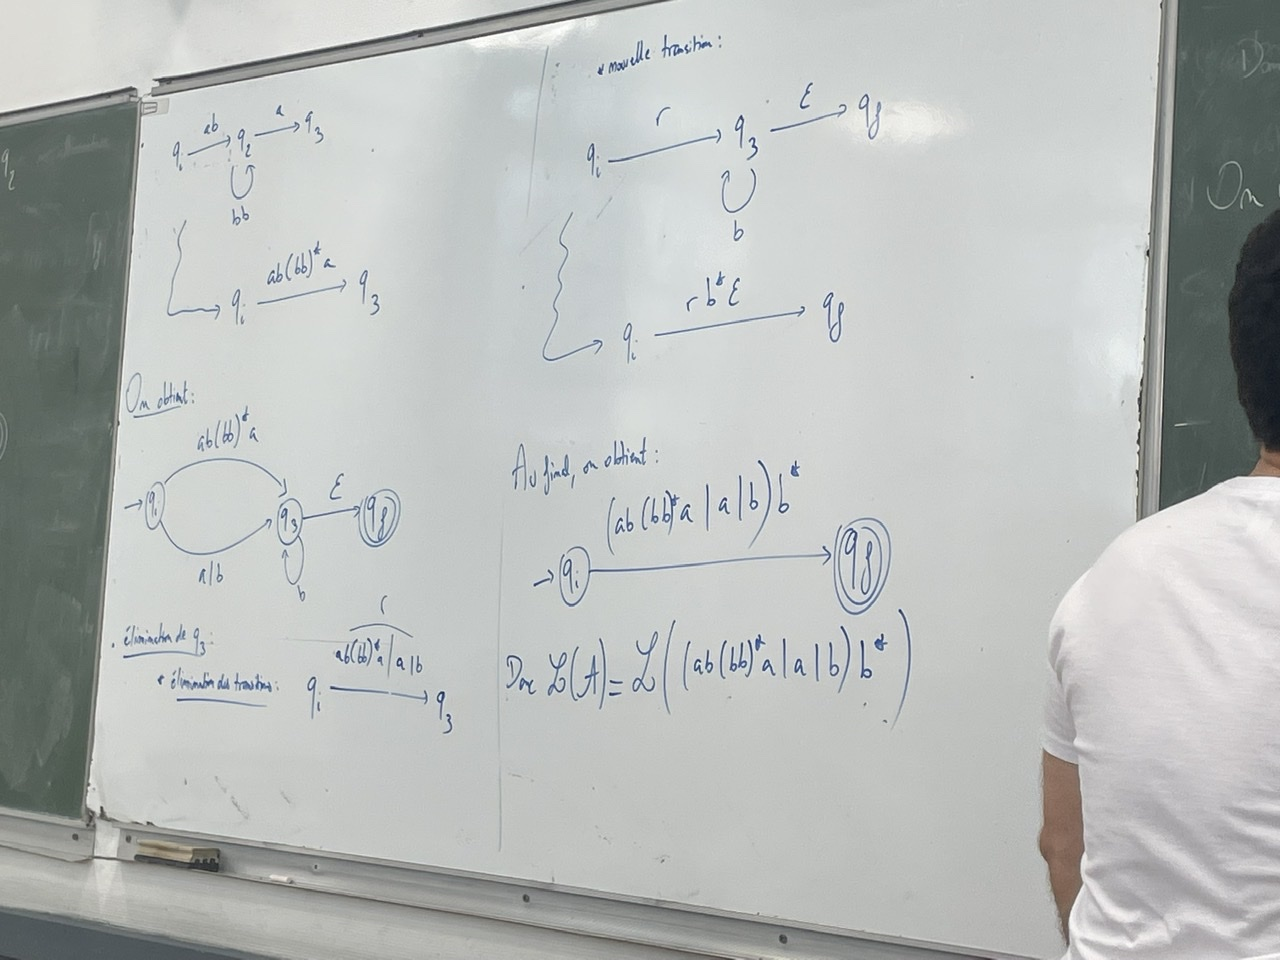
\includegraphics[scale=0.2]{Dessin/Tableau4.jpeg}
        
        
    \end{example}
    
    On remarquera les points suivants :
    %
    \begin{enumerate}
        \itt L'expression obtenue peut varier selon l'ordre dans lequel on traite les états.
        
        \itt L'expression obtenue peut être de taille exponentielle en le nombre d'états de $\bcA$.
    \end{enumerate}
    
    \subsection{Propriétés des langages reguliers}
        Une fois le lien etabli entre les language regulier et automates on peut montrer facilement certiane propriete des language regulier 
        
    \begin{theorem}{Stabilité par complémentaire}{}
        Soit $L \in \Reg_\Sigma$. Alors $\overline{L} \in \Reg_\Sigma$.
    \end{theorem}
    
    \begin{nproof}
        Soit $A = \p{Q, \Sigma, q_0, F, \delta}$ tel que $\bcL\p{\bcA} = L$
        Posons $A' =  \p{Q, \Sigma, q_0, Q \backslash F, \delta}$
        
        Soit $v \in \Sigma^\star$. Comme $A$ est déterministe et complet, il existe un unique chemin $q_0 \lima{v}_A^\star q$.
    
        Ce chemin est également l'unique chemin dans $A'$ depuis $q_0$ pour $v$. On a alors :
        %
        \begin{align*}
                && v &\in L : \bcL\p{\bcA}\\
            \iff && q &\in F\\
            \iff && q &\not\in Q \backslash F\\
            \iff && v &\not\in \bcL\p{\bcA'}
        \end{align*}
        Donc $\bcL\p{\bcA'} = \overline{L}$
    
    \end{nproof}
    
    \begin{corollary}{}{}
        Soient $\p{L_1, L_2} \in \p{\Reg_\Sigma}^2$. Alors $L_1 \backslash L_2 \in \Reg_\Sigma$.
    \end{corollary}
        
    \begin{nproof}
        $L_1 \backslash L_2 = L_1 \cup \overline{L_2 \in Reg_\Sigma}$
    \end{nproof}
    
    \begin{theorem}{Stabilité par mirroir}{}
        Soit $L \in Reg_\Sigma$.
        Alors $L^R \in Reg_\Sigma$ avec $L^R \in \Reg_\Sigma$ le langage miroir de $L$.
    \end{theorem}
    
    \begin{nproof}
        Soit $\bcA = \p{Q, \Sigma, I, F, \delta}$ un NFA tel que $L = \bcL\p{\bcA}$.
        
        On pose $\bcA' = \p{Q, \Sigma, I', F', \delta'}$ avec :
        %
        \begin{enumerate}
            \itt $I' = F$
            \itt $F' = I$
            \itt $q_1 \lima{a}{}_\bcA q_2 \in \delta \iff q_2 \lima{a}{}_{\bcA'} q_1 \in \delta'$
        \end{enumerate}
        %
        Montrons que $\bcL\p{\bcA'} = L^R$. Soit $v \in \Sigma^\star$, on a :
        %
        \begin{enumerate}
            \itt si $v = \epsilon$ : $\epsilon \in L^R \iff \epsilon \in L \iff I \cap F \neq \emptyset \iff F' \cap I' \neq \emptyset \iff \epsilon \in \bcL\p{\bcA'}$
            
            \itt sinon : $v = a_1 \dots a_n$.
            Alors $v \in L^R \iff a_n \dots a_1 \in L \iff q_n \lima{a_{n}}{}_\bcA q_{n-1} \lima{a_{n-1}}{}_\bcA \dots \lima{a_1}{}_\bcA q_0$ avec $q_n \in I$ et $q_0 \in F \iff q_0 \lima{a_1}{}_{A'} q_1 \lima{a_2}{}_{A'} q_2 \dots \lima{a_n}{}_{A'} q_n$ avec $q_0 \in I'$ et $q_n \in F' \iff v \in \bcL\p{\bcA'}$
        \end{enumerate}
    \end{nproof}
    
    \subsubsection{Lemme de l'étoile}
    
    Nous allons maintenant nous intéresser à la question suivante :
    Soit $\Sigma$ un alphabet, soit $L \subseteq \Sigma^\star$. $L$ est-il régulier ?
    \begin{enumerate}
        \itt Si on trouve une expression régulière ou un automate dont le langage est $L$, alors la réponse est oui $\dots$
        \itt Si on en trouve pas
        \begin{enumerate}
            \itt soit la réponse est non
            \itt soit on a "pas assez cherché"
        \end{enumerate}
    \end{enumerate}
    Si on pense que la réponse est non, comment prouver qu'un langage n'est pas régulier ?
    
    \begin{example}{}{}
        $\Sigma = \ens{a, b}$
        \begin{enumerate}
            \itt $L_1 = \ens{a^n b^n\enstq n \equiv m \intc{2}}$
            $L_1 = \p{a^2}^\star \p{b^2}^\star \vert \p{a^2}^\star a \p{b^2}^\star b$
            donc $L_1 \in Reg_\Sigma$
            \itt $L_2 = \ens{a^n b^n \enstq n \in \bcN}$
            On va voir maintenant que $L_2 \notin Reg_\Sigma$
        \end{enumerate}
    \end{example}
    
    Voici un critère appelé lemme de l'étoile (ou pumping lemma en anglais), qui permet de montrer qu'un certain nombre de langages ne sont pas réguliers.
    
    \begin{theorem}{Lemme de l'étoile}{}
        Soit $\Sigma$ un alphabet. Soit $L \in Reg_\Sigma$
        Alors : $\exists n \in \bcN^\star$ tel que
        $\forall u \in L$ tel que $\mod{u} \geq n$,
        $\exists \p{x, y, z} \in \p{\Sigma^\star}^3$ tels que :
        \begin{enumerate}
            \itt $u = x y z$
            \itt $y \neq \epsilon$
            \itt $\mod{xy} \leq n$
            \itt $x y^\star z \subseteq L$
        \end{enumerate}
    \end{theorem}
    
    \begin{nproof}
        Soit $\bcA = \p{Q, \Sigma, q_0, F, \delta}$ tel que $L = \bcL\p{\bcA}$
        Posons $n = \mod{Q}$.
        Soit $u \in L$ tel que $\mod{u} \geq n$ : $u = q_1 \dots q_n$ avec $m \geq n$.
        Comme $u \in \bcL\p{\bcA}$, il existe un chemin :
        $q_0 \lima{a_1}{}_\bcA q_1 \lima{a_2}{}_\bcA q_2 \dots \lima{a_m}{}_\bcA q_m$ avec $q_m \in F$.
        On passe par $m=1$ états de $Q$, et $\mod{Q} = n \leq m < n + 1$.
        Donc par principe des tirroirs de Diridlet :
        $\exists i \neq j$ tels que $q_i = q_j$
        Choisissons $i$ et $j$ les plus petits possibles. On a donc un cycle de taille $j-i$ dans ce chemin. En posant
        \begin{enumerate}
            \itt $x = a_0 \dots a_{i-1}$
            \itt $y = a_i \dots a_{j-1}$
            \itt $z = a_j \dots a_m$
        \end{enumerate}
        on a
        \begin{enumerate}
            \itt $u = x y z$
            \itt $y \neq \epsilon$ (car $i<j$)
            \itt $\mod{xy} \leq n$ car $i$ et $j$ ont été choisis les plus petits possibles, donc tous les $q_k$ pour $k \in \iint{0, j - 1}$ sont distincs 2 à 2, donc $j \leq n = \mod{Q}$
        \end{enumerate}
        On a donc un chemin ;
        $q_0  \lima{x}{}_\bcA^\star q_i = q_j \lima{z}{}^\star q_n \in F$
        %boucle en dessous du qi = qj
        Donc $\forall k \in \bcN, q_0 \lima{x y^k z}{}_\bca^\star q_m \in F$
        ie $xy^kz \in \bcL\p{\bcA} = L$
        donc $xy^kz \subseteq L$
    \end{nproof}
    On remarque que en général, on utilise le terme de l'étoile de la manière suivante :
    \begin{enumerate}
        \item On veut montrer qu'un langage $L \subseteq \Sigma^\star$ n'est pas régulier
        \item Par l'absurde, on suppose que $L$ est régulier
        \item D'après le lemme de l'étoile, $\exists n \in \bcN^\star$ tel que ...
        \item On choisis "intelligemment" un $u \in L$ tel que $\mod{u} \leq n$
        \item On montre que, \emph{pour tout} découpage possible $u = x y z$ avec $\mod{xy} \leq n$ et $y \neq \epsilon$ on a pas $x y^\star z \subseteq L$ : absurde.
        \item donc $L$ n'est pas régulier
    \end{enumerate}
    
    \begin{theorem}{}{}
        Le langage $L = \ens{a^n b^n \enstq n \in \bcN}$ n'est pas régulier.
    \end{theorem}
    
    \begin{nproof}
        Par l'absurde, on suppose que $L$ est régulier. D'après le lemme de l'étoile : $\exists n \in \bcN^\star$ tel que $\mod{u} \geq n$...
        Considérons $u = a^n b^n$
        Soit $u = x y z$ tel que $y \neq \epsilon$ et $\mod{xy} \leq n$
        Donc $\exists  \p{i, j} \in \bcN^2$ tel que
        \begin{enumerate}
            \itt $x = a^i$
            \itt $y =a^j \p{j > 0}$
            \itt $z = a^{n-i-j} b^n$
        \end{enumerate}
        et $x y^\star z \subseteq L$
        ie $\forall x \in \bcN \quad a y^\star z \in L$ en particulier $x y^0 z \in L$
        Donc $a^{n-j} b^n \in L$
        avec $j>0$ \emph{absurde} car $n-j neq n$
        donc $L$ n'est pas régulier
    \end{nproof}
    
    \begin{warning}{}{}
        Il ne faut pas s'embrouiller sur la manière dont les quantificateurs alternent : si on prend la contraposée du lemme de l'étoile, on a :
        %
        Si $\forall n \in \bdN^\star$, $\exists u \in L$ tel que $\mod{u} \geq ,$
        
        et $\forall \p{x, y, z} \in \Sigma^\star$ tel que $u = xyz$, $y \neq \epsilon$, $\mod{xy} \leq n$ et $\exists k \in \bdN$ tel que $xy^kz \not\in L$
        
        alors $L$ n'est pas régulier.
        
        Autrement dit :
        %
        \begin{enumerate}
            \itt On ne choisit pas le $n$ ;
            \itt on peut ensuite choisir $u$ comme o veut en fonction de $n$, parmi les $u \in L$ tel que $\mod{u} \geq n$
            
            \itt On doit considérer \bf{tous} les découpages possibles :
            %
            $u = xyz$ avec $\mod{xy} \leq n$ et $y \neq \epsilon$.
            
            Ainsi il vaut mieux \guill{bien choisir} $u$ pour que tous les découpages possibles se ressemblent. 
            
            \itt On peut choisir $k$ comme on veut pour que $xy^kz \not\in L$.
        \end{enumerate}
    \end{warning}
    
    Parfois, pour montrer qu'un langage $L$ n'est pas régulier, il est plus facile de raisonner sur un autre langage $L'$ dépendant de $L$, tel que $L \in \Reg_\Sigma \implies L' \in \Reg_\Sigma$.
    
    On montre alors, en vertu du lemme de l'étoile, que $L'$ n'est pas régulier et donc que $L$ n'est pas régulier.
    %
    \begin{example}{}{}
        On considère $\hg{L = \ens{a^nb^n \enstq n \neq m}}$.
        
        Si $L$ était régulier, alors $a^\star b^\star \backslash L$ serait régulier. Or :
        %
        \[ a^\star b^\star \backslash L = \ens{a^nb^n \enstq n = m} = \ens{a^nb^n \enstq n \in \bdN}\]
        %
        n'est pas régulier d'après le théorème précédent.
    \end{example}
    
    Les langages réguliers (et les automates) sont donc très utiles pour chercher des motifs simples dans un texte. On souhaiterait s'en servir pour effectuer une analyse syntaxique du code source d'un programme. Par exemple, trouver tous les mots clés (\texttt{while}, \texttt{for}, \texttt{if}, \texttt{float}, \texttt{float}, \dots) du langage de programmation dans le code source est faisable à l'aide d'un automate. Mais qu'en est-il d'autres propriétés à vérifier ? Par exemple, peut-on vérifier si les expressions présentes dans le code source sont bien parenthésées ?
    
    Pour étudier ce problème, étudions l'exercice suivant :
    %
    \begin{exercise}{}{}
        $\Sigma = \ens{(, ), [, ], \{, \}, <, >}$
        %
        $L = \ens{u \in \Sigma^\star \enstq u \ \text{est bien parenthésé}}$ est-il régulier ?
    \end{exercise}
\end{document}
